% Notes on 4-class, Q-antipodal, preservation of semidefinite cone.
%
%  B G Kodalen,  W J Martin

\documentclass[12pt]{article}

\usepackage{graphicx,amsthm,fullpage} 
\usepackage{amssymb}
\usepackage{amsfonts}
\usepackage{amsmath}
\usepackage{enumitem}
\usepackage{tabularx}



\newcommand{\BMA}{\mathbb{A}}
\newcommand{\BMB}{\mathbb{B}}
\newcommand{\ints}{\mathbb{Z}}
\newcommand{\rats}{\mathbb{Q}}
\newcommand{\re}{\mathbb{R}}
\newcommand{\cx}{\mathbb{C}}
\newcommand{\FF}{\mathbb{F}}
\newcommand{\cB}{\mathcal{B}}
\newcommand{\bb}{\mathbf{b}}
\newcommand{\bw}{\mathbf{w}}
\newcommand{\bx}{\mathbf{x}}
\newcommand{\sA}{\mathsf{A}}
\newcommand{\sB}{\mathsf{B}}
\newcommand{\sF}{\mathsf{F}}
\newcommand{\cC}{\mathcal{C}}
\newcommand{\cG}{\mathcal{G}}
\newcommand{\bbL}{\mathbb{L}}
\newcommand{\cM}{\mathcal{M}}
\newcommand{\cN}{\mathcal{N}}
\newcommand{\cR}{\mathcal{R}}
\newcommand{\cS}{\mathcal{S}}
\newcommand{\sS}{\mathsf{S}}
\newcommand{\ones}{\mathbf{1}}

\DeclareMathOperator{\tr}{tr}
\DeclareMathOperator{\spn}{span}
\DeclareMathOperator{\rank}{rank}
\DeclareMathOperator{\srg}{srg}
\DeclareMathOperator{\Mat}{\mathsf{Mat}}

\newenvironment{my_enumerate}{
\begin{enumerate}
  \setlength{\itemsep}{1pt}
  \setlength{\parskip}{0pt}
  \setlength{\parsep}{0pt}}{\end{enumerate}
}


\newtheorem{thm}{Theorem}[section]
\newtheorem{lem}[thm]{Lemma}
\newtheorem{prop}[thm]{Proposition}
\newtheorem{cor}[thm]{Corollary}
\newtheorem{example}{Example}[section]




\title{\textbf{Cometric Association Schemes}}
\author{Brian G. Kodalen}
\date{}
\begin{document}
	\maketitle
	\vspace{3cm}
	\begin{center} A dissertation for the degree of\\Doctor of Philosophy.\\
		\vspace{1cm}
		Mathematical Sciences Department\\Worcester Polytechnic Institute\\\today\end{center}
	\vspace{3cm}
	\textbf{PhD Committee Members:}
	\begin{itemize}[label={}]
		\itemsep-.5em
		\item Dr. Peter J. Cameron, Queen Mary, University of London
		\item Dr. Padraig \'{O} Cath\'{a}in, WPI
		\item Dr. Peter R. Christopher, WPI
		\item Dr. William M. Kantor, University of Oregon
		\item Dr. William J. Martin, WPI (Advisor)
		\item Dr. G\'{a}bor N. S\'{a}rk\"{o}zy, WPI
	\end{itemize}
\newpage
\tableofcontents
\newpage
\listoffigures
\newpage
\section*{List of Symbols}\label{los}
\begin{tabularx}{\textwidth}{| X | X |}
\hline
	$\BMA$ & Algebras\\\hline
	$u,v,w$ & Vectors\\
	\hspace{2mm} $a,b,c$ & \\\hline
	$\mathcal{R}$ & Set of Relations\\\hline
	$X$ & Set of points\\\hline
	$G$, $G_X$ & Gram matrix/Gram matrix of point set $X$\\\hline
	$Q_k(t)$ & Gegenbauer polynomial with degree $k$\\\hline
	$P,Q$ & First and second Eigenmatrices\\\hline
	$\succeq$ & Positive semi-definite\\\hline
	$\mathbb{R},\mathbb{Z},\mathbb{Q}$, etc.&Reals, Integers, Rationals, etc.\\\hline
	$\scR$& Ring\\\hline
	$J,J_{n\times m}$& All ones matrix\\\hline
	$e_0,e_1,\dots,e_d$& standard basis vectors\\\hline
	$\ones$ & All ones vector\\\hline
	&\\\hline
	&\\\hline
	&\\\hline
	&\\\hline
	&\\\hline
	&\\\hline
\end{tabularx}
\section{Introduction}
\include{Introduction}
\section{Association schemes}
	\chapter{Association schemes}\label{association}
	Association schemes arise in group theory, graph theory, design theory, coding theory and more. For example, if $X$ is a finite group with conjugacy classes $\cC[g] = \{hgh^{-1}:h\in X\}$ ($g\in X$), then the conjugacy class relations $R_g = \left\{ (a,b) \mid ab^{-1} \in \cC[g]  \right\}$ yield a 
	commutative association scheme on the vertex set $X$. The orbits on $X\times X$ of any 
	permutation group $G$ acting generously transitively on a set $X$  give a symmetric association scheme.
	Some of the most well-studied association schemes are distance-regular graphs, including Moore graphs, distance-transitive graphs, strongly regular graphs, generalized polygons, etc. One studies 
	$q$-ary error-correcting codes of length $n$ as vertex subsets of the Hamming association scheme
	$H(n,q)$ \cite[Sec.~9.2]{Brouwer1989} and $t$-($v,k,\lambda$) designs as vertex subsets of the 
	Johnson association scheme  $J(v,k)$ \cite[Sec.~9.1]{Brouwer1989}.  For an introduction to the 
	extensive literature on the subject, the reader may consult \cite{Delsarte1973,Bannai1984,Brouwer1989,Godsil1993}, 
	the survey \cite{Martin2009}, or the more recent book of  Bailey \cite{Bailey2005} which focuses on 
	connections to the statistical design of experiments.
	\begin{definition}
	Let $X$ be a finite set of vertices. A \textit{symmetric d-class association scheme}\index{association scheme!symmetric} (see \cite{Brouwer1989}) on $X$ is a pair $(X,\mathcal{R})$ where $\mathcal{R} =\left\{R_0,R_1,\dots,R_d\right\}$ is a set of $d+1$ relations on $X$ satisfying the following properties:
	\begin{enumerate}[label=(\roman*)]
		\item $R_0$ is the identity relation;
		\item $\left\{R_0,R_1,\dots, R_d\right\}$ forms a partition of $X\times X$;
		\item $(x,y)\in R_i$ implies $(y,x)\in R_i$;
		\item for $0\leq i,j,k\leq d$ there exist constants $p_{i,j}^k$ such that for any $(x,y)\in R_k$, the number of vertices $z$ for which $(x,z)\in R_i$ and $(z,y)\in R_j$ is equal to $p_{i,j}^k$ independent of our original choice of $x$ and $y$.
	\end{enumerate}
	\end{definition}
	The constants $p_{i,j}^k$ are known as the \emph{intersection numbers}\index{parameters!intersection numbers} of our association scheme and we allow ourselves to suppress the comma whenever $i$ and $j$ are given by single digits, thus $p_{0,7}^6$ and $p_{07}^6$ are synonymous throughout this thesis. Property $(iii)$ and $(iv)$ together imply that $p_{ij}^k = p_{ji}^k$ for all $i,j,k$; we call such an association scheme \textit{commutative}. There is a broader definition for a \emph{commutative association scheme}\index{association scheme!commutative} where we replace $(iii)$ with the requirement that for every $i$, there exists some $j$ such that $R_j = R_i^T$; that is $(x,y)\in R_i$ if and only if $(y,x)\in R_j$. In this case however, we add the additional requirement $p_{ij}^k = p_{ji}^k$. Throughout this thesis, all association schemes will be symmetric, though we will add remarks at times when the theorems apply directly to the non-symmetric case as well.
	
	For each $0\leq i\leq d$ we define the (undirected) graph $\Gamma_i = \Gamma(X,R_i)$ on $X$ with $\Gamma_1,\dots,\Gamma_d$ all simple. For each $a\in X$ we define the $i^\text{th}$ \emph{neighborhood}\index{relation!neighborhood} of $a$ $R_i(a) = \left\{b\in X\vert (a,b)\in R_i\right\}$; i.e. $R_i(a)$ is the neighborhood of $a$ in the graph $\Gamma_i$. Then for any $a\in X$, the set $X$ is partitioned into the \emph{subconstituents}\index{relation!subconstituents} $R_i(a)$ for $0\leq i\leq d$. Consider the following example on $8$ vertices:
	\begin{example} The following association scheme is known as the \emph{3-cube}\index{3-cube} with vertex set $X = \left\{0,\dots,7\right\}$ and relations corresponding to the graphs $\Gamma_0,\dots,\Gamma_3$ given below.
		\begin{figure}[H]\begin{center}\scalebox{.7}{$\begin{aligned}
		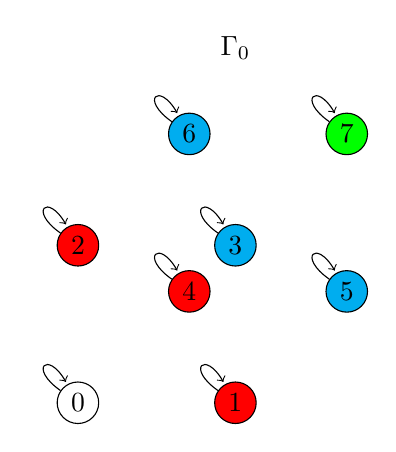
\begin{tikzpicture}[shorten >=1pt,auto,node distance=2cm,
		thin,main node/.style = {circle,draw, inner sep = 0pt, minimum size = 15pt}]
		
		\node[main node,fill=white] (1) {0};
		\node[main node,fill=red] [right of = 1](2) {1};
		\node[main node,fill=red] [above of = 1](3) {2};
		\node[main node,fill=cyan] [right of = 3](4) {3};
		\node[main node,fill=red] [above right of = 1](5) {4};
		\node[main node,fill=cyan] [right of = 5](6) {5};
		\node[main node,fill=cyan] [above of = 5] (7) {6};
		\node[main node,fill=green] [right of = 7](8) {7};
		\node at (2,4.5) (9) {$\Gamma_0$};
		
		\path (1) edge [in=120,out=145,loop] ();
		\path (2) edge [in=120,out=145,loop] ();
		\path (3) edge [in=120,out=145,loop] ();
		\path (4) edge [in=120,out=145,loop] ();
		\path (5) edge [in=120,out=145,loop] ();
		\path (6) edge [in=120,out=145,loop] ();
		\path (7) edge [in=120,out=145,loop] ();
		\path (8) edge [in=120,out=145,loop] ();
		
		\end{tikzpicture}\qquad&\qquad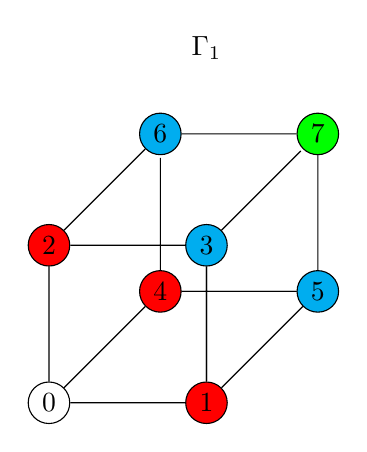
\begin{tikzpicture}[shorten >=1pt,auto,node distance=2cm,
		thin,main node/.style = {circle,draw, inner sep = 0pt, minimum size = 15pt}]
		
		\node[main node,fill=white] (1) {0};
		\node[main node,fill=red] [right of = 1](2) {1};
		\node[main node,fill=red] [above of = 1](3) {2};
		\node[main node,fill=cyan] [right of = 3](4) {3};
		\node[main node,fill=red] [above right of = 1](5) {4};
		\node[main node,fill=cyan] [right of = 5](6) {5};
		\node[main node,fill=cyan] [above of = 5] (7) {6};
		\node[main node,fill=green] [right of = 7](8) {7};
		\node at (2,4.5) (9) {$\Gamma_1$};
		
		\draw[-] (3)--(1)--(2)--(4)--(3)--(7)--(8)--(6)--(5)--(7);
		\draw[-] (1)--(5)--(6)--(2)--(4)--(8);
		\end{tikzpicture}\qquad\qquad
		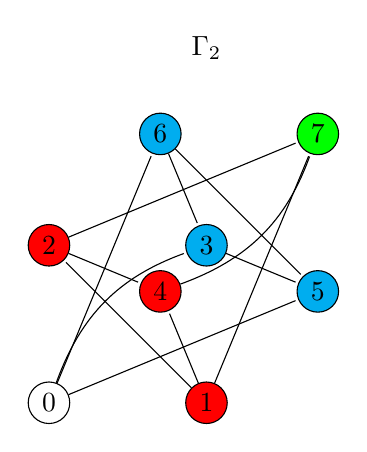
\begin{tikzpicture}[shorten >=1pt,auto,node distance=2cm,
		thin,main node/.style = {circle,draw, inner sep = 0pt, minimum size = 15pt}]
		
		\node[main node,fill=white] (1) {0};
		\node[main node,fill=red] [right of = 1](2) {1};
		\node[main node,fill=red] [above of = 1](3) {2};
		\node[main node,fill=cyan] [right of = 3](4) {3};
		\node[main node,fill=red] [above right of = 1](5) {4};
		\node[main node,fill=cyan] [right of = 5](6) {5};
		\node[main node,fill=cyan] [above of = 5] (7) {6};
		\node[main node,fill=green] [right of = 7](8) {7};
		\node at (2,4.5) (9) {$\Gamma_2$};
		
		\path[-]
		(1)edge [bend left=25] node {} (4)
		edge node {} (6)
		edge node {} (7)
		(2)edge node {} (3)
		edge node {} (5)
		edge node {} (8)
		(3)edge node {} (5)
		edge node {} (8)
		(4) edge node {} (6)
		(7) edge node {} (4)
		edge node {} (6)
		(5) edge [bend right = 25] node {} (8);
		\end{tikzpicture}\qquad&\qquad
		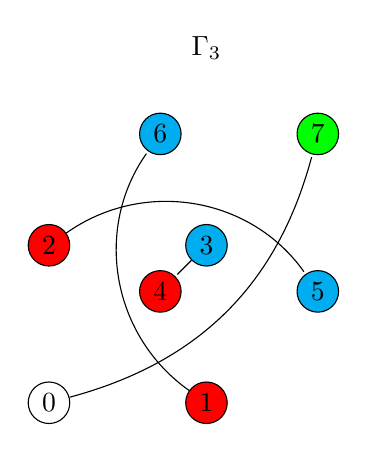
\begin{tikzpicture}[shorten >=1pt,auto,node distance=2cm,
		thin,main node/.style = {circle,draw, inner sep = 0pt, minimum size = 15pt}]
		
		\node[main node,fill=white] (1) {0};
		\node[main node,fill=red] [right of = 1](2) {1};
		\node[main node,fill=red] [above of = 1](3) {2};
		\node[main node,fill=cyan] [right of = 3](4) {3};
		\node[main node,fill=red] [above right of = 1](5) {4};
		\node[main node,fill=cyan] [right of = 5](6) {5};
		\node[main node,fill=cyan] [above of = 5] (7) {6};
		\node[main node,fill=green] [right of = 7](8) {7};
		\node at (2,4.5) (9) {$\Gamma_3$};
		
		\path[-]
		(1) edge [bend right] node {} (8)
		(2) edge [bend left=45] node {} (7)
		(3) edge [bend left=45] node {} (6)
		(4) edge node {} (5);
		\end{tikzpicture}
		\end{aligned}$}\end{center}
		\caption[Graphs of the 3-cube.]{The four graphs of the 3-cube. The four subconstituents of the vertex $0$ are colored white, red, blue, and green respectively.}\label{3cube}
		\end{figure}
		The intersection numbers of this association scheme are as follows where the $i^\text{th}$ matrix list $p^k_{ij}$ with rows indexed by $k$ and columns indexed by $j$:
		\[\left[\begin{array}{cccc}
		1&0&0&0\\
		0&1&0&0\\
		0&0&1&0\\
		0&0&0&1\\
		\end{array}\right],\quad\left[\begin{array}{cccc}
		0&3&0&0\\
		1&0&2&0\\
		0&2&0&1\\
		0&0&3&0\\
		\end{array}\right],\quad\left[\begin{array}{cccc}
		0&0&3&0\\
		0&2&0&1\\
		1&0&2&0\\
		0&3&0&0\\
		\end{array}\right],\quad\left[\begin{array}{cccc}
		0&0&0&1\\
		0&0&1&0\\
		0&1&0&0\\
		1&0&0&0\\
		\end{array}\right].\]
		Since $p^k_{ij} = p^k_{ji}$, many of the columns listed above are redundant, thus we may instead give a more brief list of the intersection numbers as follows:
		\[\begin{array}{c|cccc|ccc|cc|c}
		j & p^{j}_{0,0}	&p^{j}_{0,1}& p^{j}_{0,2} 	& p^{j}_{0,3}   & p^{j}_{1,1}	&p^{j}_{1,2}& p^{j}_{1,3} 	& p^{j}_{2,2} 	& p^{j}_{2,3} 	& p^{j}_{3,3}\\\hline
		0 & 1			& 0			& 0 			& 0				& 3				& 0			& 0 			& 3				& 0   			& 1\\
		1 & 0			& 1			& 0 			& 0				& 0				& 2			& 0 			& 0   			& 1   			& 0\\
		2 & 0			& 0			& 1 			& 0				& 2				& 0 		& 1				& 2 			& 0 			& 0\\
		3 & 0			& 0			& 0 			& 1				& 0 			& 3			& 0 			& 0   			& 0 			& 0\\
		\end{array}\]
		We often find this brief description useful and will further reduce our description of the parameters in many of the examples whenever possible.
	\end{example}
	For any $0\leq i\leq d$ and any vertex $x\in X$,
	\[p^{0}_{ii} = \left\vert\left\{y:(y,x)\in R_i\right\}\right\vert = \left\vert R_i(x)\right\vert.\]
	Thus we define $k_i:=p^0_{ii}$ as the \emph{valency}\index{valency} of the $i^\text{th}$ relation. Many other restrictions on our intersection numbers follow immediately from our definition, for instance $p^0_{12} = 0$; we will summarize these in a latter lemma.
	\section{Bose-Mesner algebra}
	Often it becomes useful to order the vertices in $X$ and then represent each $R_i$ as a 01-matrix $A_i$ where the $(x,y)$ entry of $A_i$ is 1 if and only if $(x,y)\in R_i$, thus $A_i$ is the adjacency matrix of $\Gamma_i$. The defining properties of an association scheme are then encoded as:
	\begin{enumerate}[label=(\roman*)]
		\item $A_0 = I$;
		\item $\sum_i A_i = J$;
		\item for all $0\leq i\leq d$, $A_i^T = A_i$;
		\item for all $0\leq i,j\leq d$, $A_iA_j = \sum p_{ij}^k A_k$.
	\end{enumerate}
	The fourth condition tells us that $\BMA = \text{span}\left\{A_0,A_1,\dots A_d\right\}$\index{01-basis} forms a matrix algebra under standard matrix multiplication. We call this algebra the \emph{Bose-Mesner algebra}\index{Bose-Mesner algebra} and note that the remaining conditions ensure it is a $(d+1)$-dimensional algebra of symmetric matrices containing the identity. Further, as our basis matrices are 01-matrices with disjoint support, this algebra is also closed under Schur (element-wise) products and contains the Schur identity, $J$. We find that the existence of such an algebra is also sufficient to define an association scheme; that is, any $(d+1)$-dimensional matrix algebra closed under both standard and Schur matrix products containing the identities for both operations corresponds to the Bose-Mesner algebra of some association scheme. In many of the chapters that follow, we will use this to show the existence or non-existence of an association scheme, focusing on the algebraic definition instead of the combinatorics. Recall that a commutative association scheme was defined as one in which $p^k_{ij} = p^k_{ji}$ for all $i,j,k$. In this setting this property tells us that $A_iA_j = A_jA_i$; that is, our algebra is commutative. Therefore, we may simultaneously diagonalize the matrices $\left\{A_0,\dots,A_d\right\}$ using the maximal common orthogonal eigenspaces $V_0,\dots,V_{d'}$ with corresponding idempotents $E_0,\dots,E_{d'}$. Since, for every $i$, there exists eigenvalues $\theta_{ij}$ such that $A_i = \sum_{j=0}^{d'}\theta_{ij}E_j$ we find that $\BMA \subseteq \text{span}\left\{E_0,E_1,\dots, E_{d'}\right\}$ thus $d\leq d'$. Further since the eigenspaces $V_j$ are maximal for each $0\leq j\leq d$ and pairwise orthogonal,
	\[E_j = \frac{1}{c_j}\prod_{i=0}^d\left(\prod_{\theta_{ik}\neq\theta_{ij}}\left(A_i-\theta_{ik}I\right)\right)\]
	for some normalization constant $c_j$. Thus $E_j\in \BMA$ giving $\text{span}\left\{E_0,E_1,\dots, E_{d'}\right\}\subseteq\BMA$\index{idempotent basis} and therefore $d=d'$. Then, $\BMA$ contains a basis of $d+1$ idempotents $E_0,\dots,E_d$ which diagonalize every matrix in $\BMA$ and act as projection matrices onto the common eigenspaces. Since the rank 1 idempotent $J\in\BMA$, we find that $\frac{1}{\vert X\vert}J$ must be contained within this basis; by convention we assume $E_0= \frac{1}{\vert X\vert}J$. We take a moment here to remark on the notion of duality in our matrix algebra. We have already mentioned that $\BMA$ is closed under two distinct products: standard matrix multiplication and Schur multiplication. While it is clear these are distinct products, consider an abstract vector space with basis vectors $\left\{b_i\right\}$. For any pair of vectors $v = \sum_i v_ib_i$ and $w = \sum_i w_ib_i$, we may define the \emph{product with respect to basis $\left\{b_i\right\}$} as $v\star w = \sum_i (v_iw_i)b_i$. In this light, our two distinct products become very similar; for $F,F'\in\BMA$ with $F = \sum_if_iE_i = \sum_i g_iA_i$ and $F' = \sum_if_i'E_i = \sum_i g_i'A_i$, we have
	\[\begin{aligned}
	FF' & =\sum_i\sum_jf_if_j'E_iE_j = \sum_i f_if_i'E_i,\\
	F\circ F' &=\sum_i\sum_jg_ig_i'A_i\circ A_j= \sum_i g_ig_i'A_i.
	\end{aligned}\]
	Therefore our two products may be described as the product with respect to the basis $\left\{E_i\right\}$ (standard matrix multiplication) and the product with respect to the basis $\left\{A_i\right\}$ (elementise multiplication). Thus we consider our two products similar and will often refer to them as dual operations on our algebra. Further, we consider the basis matrices $A_0,\dots,A_d$ and $E_0,\dots,E_d$ dual bases. Throughout this thesis, we will often be interested in investigating this duality and pointing out when there are differences and/or gaps in our understanding of the landscape. Our first consideration regarding these two bases for our algebra is the change of basis matrices between the two. Since both $\left\{A_0,\dots,A_d\right\}$ and $\left\{E_0,\dots,E_d\right\}$ form bases for $\BMA$, there exist unique matrices $P$ and $Q$ so that
	\begin{equation}
	\label{PQmat}
	A_i = \sum_{j} P_{ji} E_j,\qquad E_j = \frac{1}{\vert X\vert} \sum_{i} Q_{ij}A_i.
	\end{equation}
	We call $P$ and $Q$ the \emph{first and second eigenmatrices}\index{eigenmatrices}, noting that column $i$ of $P$ gives the eigenvalues of $A_i$ while column $j$ of $Q$ gives the ``dual eigenvalues"\index{idempotent basis!dual eigenvalues} of $\vert X\vert E_j$---eigenvalues with respect to the Schur product. Let $\Delta_m=\text{diag}(m_0,m_1,\dots,m_d)$ and $\Delta_k=\text{diag}(k_0,k_1,\dots,k_d)$ and the following two relations hold for our eigenmatrices:
	\begin{lem}[\cite{Brouwer1989}, First and second orthogonality relations] \label{orthorels}\index{eigenmatrices!orthogonality relations}The eigenmatrices of an association scheme satisfy:
		\begin{equation}
		PQ = \vert X\vert I, \qquad \Delta_mP = Q^T\Delta_k
		\end{equation}
	\end{lem}
	A second consideration for our dual bases is that while we used the existence of structure constants $p^k_{ij}$ to show that $\BMA$ was closed under matrix multiplication, closure under Schur products came from the fact that each $A_i$ was idempotent under this product. This additional closure implies the existence of structure constants for our second basis. Thus, for $0\leq i,j,k\leq d$ there exists constants $q^k_{ij}$ so that
	\begin{equation}E_i\circ E_j = \frac{1}{\vert X\vert}\sum_k q_{ij}^k E_k.\label{Emult}\end{equation}
	We call these constants the \emph{Krein paramters}\index{parameters!Krein} of the association scheme. Here we list many of the properties of both the intersection numbers and the Krein parameters, including our first and second eigenmatrices as well. See Lemmas 2.1.1, 2.2.1, 2.3.1, and Theorem 2.3.2 for proofs of the following lemma. One may observe the dual nature of the intersection numbers and the Krein parameters from this lemma.
	\begin{lem}[{\cite{Brouwer1989}}]\label{kitchensink} The parameters $p^\ell_{ij}$, $q^\ell_{ij}$, $k_i = p^0_{ii}$, $m_j = q^0_{jj}$, and the eigenmatrices $P$ and $Q$ satisfy:
		\begin{multicols}{2}
		\begin{enumerate}
			\item[(i)] $\displaystyle{p_{0j}^\ell = \delta_{j\ell}}$,
			\item[(ii)] $\displaystyle{p^0_{ij} = \delta_{ij}k_i}$,
			\item[(iii)] $\displaystyle{p^\ell_{ij} = p^\ell_{ji}}$,
			\item[(iv)] $\displaystyle{p^\ell_{ij}k_\ell= p^j_{i\ell}k_j}$,
			\item[(v)] $\displaystyle{\sum_jp^\ell_{ij} = k_i}$,
			\item[(vi)] $\displaystyle{\sum_\ell p^\ell_{ij}p^m_{\ell h} = \sum_\ell p^m_{i\ell}p^\ell_{jh}}$,
			\item[(vii)] $\displaystyle{P_{ij}P_{ih} = \sum_\ell p^\ell_{jh}P_{i\ell}}$,
			\item[(viii)] $\displaystyle{P_{ji}Q_{hj} = \sum_\ell p_{i\ell}^hQ_{\ell j}}$,
			\item[(ix)] $\displaystyle{\sum_{j}P_{ji} = \sum_{h}p^h_{hi}}$,
			\item[(x)] $\displaystyle{P_{j0} = 1}$,
			\item[(xi)] $\displaystyle{P_{0i} = k_i}$,
			\item[(xii)] $\displaystyle{\sum_j m_jP_{ji}P_{jh} = \vert X\vert k_i\delta_{ih}}$,
			\item[(xiii)] $\displaystyle{p^\ell_{ij} = \frac{1}{\vert X\vert k_\ell}\sum_{h=0}^d m_hP_{hi}P_{h j}P_{h\ell}}$,
				
			\item[($i^\prime$)] $\displaystyle{q^\ell_{0j} = \delta_{j\ell}}$,
			\item[($ii^\prime$)] $\displaystyle{q^0_{ij} = \delta_{ij}m_j}$,
			\item[($iii^\prime$)] $\displaystyle{q^{\ell}_{ij} = q^\ell_{ji}}$,
			\item[($iv^\prime$)] $\displaystyle{q^\ell_{ij}m_\ell = q^j_{i\ell}m_j}$,
			\item[($v^\prime$)] $\displaystyle{\sum_j q^\ell_{ij} = m_i}$,
			\item[($vi^\prime$)] $\displaystyle{\sum_\ell q^\ell_{ij}q^{m}_{\ell h} = \sum_\ell q^m_{i\ell}q^\ell_{jh}}$,
			\item[($vii^\prime$)] $\displaystyle{Q_{ij}Q_{ih} = \sum_{\ell}q^\ell_{jh}Q_{i\ell}}$,
			\item[($viii^\prime$)] $\displaystyle{P_{ij}Q_{jh} = \sum_\ell q^i_{h\ell}P_{\ell j}}$,
			\item[($ix^\prime$)] $\displaystyle{\sum_{j}Q_{ji} = \sum_{h}q^h_{hi}}$,
			\item[($x^\prime$)] $\displaystyle{Q_{i0} = 1}$,
			\item[($xi^\prime$)] $\displaystyle{Q_{0j} = m_j}$,
			\item[($xii^\prime$)] $\displaystyle{\sum_i k_iQ_{ij}Q_{ih} = \vert X\vert m_j\delta_{jh}}$,
			\item[($xiii^\prime$)] $\displaystyle{q^\ell_{ij} = \frac{1}{\vert X\vert m_\ell}\sum_{h=0}^d k_hQ_{hi}Q_{h j}Q_{h\ell}}$.
			
		\end{enumerate}
		\end{multicols}
	\end{lem}
	\section{Parameter arrays}
	For a matrix $A$, we denote the entry in row $i$ and column $j$ as $\left[A\right]_{ij}$. We define the \emph{arrays of intersection numbers}\index{parameters!arrays of intersection numbers} $L_0,\dots,L_d$ as $(d+1)\PLH(d+1)$ matrices with $\left[L_i\right]_{kj} = p^k_{ij}$. We then define the vector space $\bbL = \text{span}\left\{L_0,\dots,L_d\right\}$ and note that Lemma \ref{kitchensink} $(vi)$ gives us
	\[
	\left[L_iL_j\right]_{mk} = \sum_lp^m_{il}p^l_{jk} = \sum_{l}p^l_{ij}p^m_{lk} = \sum_l p^l_{ij}\left[L_l\right]_{mk}
	\]
	for $0\leq m,k\leq d$. Therefore we find that this vector space forms a matrix algebra under matrix multiplication with
	\begin{equation}\label{Lprod}
	L_iL_j = \sum_l p^l_{ij}L_l.
	\end{equation}
	Likewise, we define the \emph{arrays of Krein parameters}\index{parameters!arrays of Krein parameters} as $L_0^*,\dots,L_d^*$ with $\left[L_i^*\right]_{kj} = q^k_{ij}$. This provides a dual matrix algebra $\bbL^* = \text{span}\left\{L_0^*,\dots,L_d^*\right\}$ as Lemma \ref{kitchensink} $(vi^\prime)$ gives
	\begin{equation}\label{Lstarprod}
	L_i^*L_j^* = \sum_{l}q^l_{ij}L_l^*.
	\end{equation}
	In both cases, we define an algebra isomorphism $\phi:\BMA\rightarrow\bbL$ or $\phi^*:\BMA\rightarrow\bbL^*$ via the basis mappings
	\begin{equation}
		\phi(A_i) = L_i\qquad \phi^*(E_i) = \frac{1}{\vert X\vert}L_i^*.
	\end{equation}
	The first isomorphism preserves standard matrix multiplication while the second preserves Schur products. This provides us with the following Lemma.
	\begin{lem}\label{arrayeigenvec}
		Let $P$ and $Q$ be the first and second eigenmatrices of an association scheme with the arrays of intersection numbers $L_0,\dots,L_d$ and arrays of Krein parameters $L_0^*,\dots,L_d^*$. Then column $j$ of $Q$ is an eigenvector of $L_i$ with eigenvalue $P_{ji}$. Likewise column $i$ of $P$ is an eigenvector of $L_j^*$ with eigenvalue $Q_{ij}$.
	\end{lem}
	\begin{proof}
	Let $A_i$ be a 01-basis matrix and $E_j$ be a basis idempotent of our association scheme. Then $A_iE_j = P_{ji}E_j$ and $E_j\circ A_i = \frac{Q_{ji}}{\vert X\vert}A_i$. Noting that $E_j = \frac{1}{\vert X\vert}\sum_{j}Q_{ji} A_i$ we find that $\phi(\vert X\vert E_j) = \sum_{i}Q_{ij} L_i$ and thus
	\[P_{ji}\left(\sum_iQ_{ij}L_i\right) = \phi(\vert X\vert A_iE_j) = L_i\left(\sum_iQ_{ij}L_i\right).\]
	Similarly, $A_i = \sum_{j}P_{ji} E_j$ and thus we find that $\phi^*(\vert X\vert A_i) = \sum_{j}P_{ji} L_i^*$ giving,
	\[Q_{ji}\left(\frac{1}{\vert X\vert}\sum_jP_{ji}L_j^*\right) = \phi^*(\vert X\vert E_j\circ A_i) = L_j^*\left(\frac{1}{\vert X\vert}\sum_jP_{ji}L_j^*\right)\]
	In each case, we note that $\left[L_i\right]_{j0} = \left[L_j^*\right]_{i0} = \delta_{ij}$ and thus taking the first column of each matrix product gives our result.
	\end{proof}
	We will refer to $L_1$ as the \emph{intersection matrix}\index{parameters!intersection matrix} and $L_1^*$ as the \emph{Krein matrix}\index{parameters!Krein matrix}; these two matrices will become particularly important for polynomial schemes (see Section \ref{poly}), for which they are tridiagonal. We end this section by noting that the matrices given in Example \ref{3cube} were exactly the arrays of intersection numbers for that association scheme. A final note before moving on is that the parameters of an association scheme need not define the scheme uniquely. In fact, there exists non-isomorphic $2$-class association schemes with exactly the same parameters--consider the $4\times 4$ rook graph and Shrikhande graph.
	\section{Example Duality}\label{dualpair}
	In this section, we give an explicit example of the duality previously alluded to. Consider first the strongly regular graph given by $K_{3,3}$. This association scheme is a 2-class bipartite scheme with nontrivial relations given by adjacency in $K_{3,3}$ and non-adjacency in $K_{3,3}$ respectively. Thus the three graphs for this scheme are
		\begin{figure}[H]\begin{center}\scalebox{.7}{$\begin{aligned}
				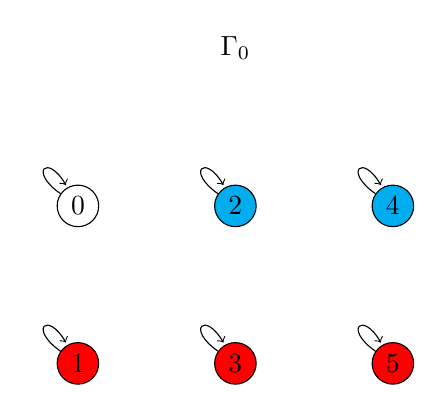
\begin{tikzpicture}[shorten >=1pt,auto,node distance=2cm,
				thin,main node/.style = {circle,draw, inner sep = 0pt, minimum size = 15pt}]
				
				\node[main node,fill=white] (1) {0};
				\node[main node,fill=cyan] [right of = 1](2) {2};
				\node[main node,fill=cyan] [right of = 2](3) {4};
				\node[main node,fill=red] [below of = 1](4) {1};
				\node[main node,fill=red] [right of = 4](5) {3};
				\node[main node,fill=red] [right of = 5](6) {5};
				\node [above of =2] (9) {$\Gamma_0$};
				
				\path (1) edge [in=120,out=145,loop] ();
				\path (2) edge [in=120,out=145,loop] ();
				\path (3) edge [in=120,out=145,loop] ();
				\path (4) edge [in=120,out=145,loop] ();
				\path (5) edge [in=120,out=145,loop] ();
				\path (6) edge [in=120,out=145,loop] ();
				
				\end{tikzpicture}\qquad&\qquad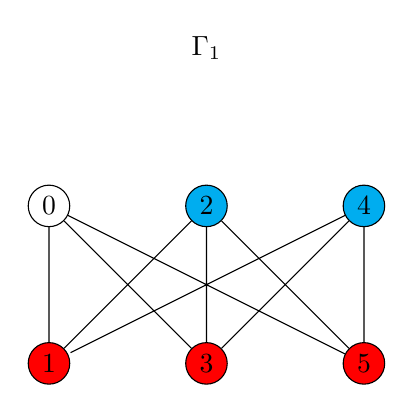
\begin{tikzpicture}[shorten >=1pt,auto,node distance=2cm,
				thin,main node/.style = {circle,draw, inner sep = 0pt, minimum size = 15pt}]
				
				\node[main node,fill=white] (1) {0};
				\node[main node,fill=cyan] [right of = 1](2) {2};
				\node[main node,fill=cyan] [right of = 2](3) {4};
				\node[main node,fill=red] [below of = 1](4) {1};
				\node[main node,fill=red] [right of = 4](5) {3};
				\node[main node,fill=red] [right of = 5](6) {5};
				\node [above of =2] {$\Gamma_1$};
				
				\draw[-] (1)--(4)--(2)--(5)--(3)--(6)--(1)--(5)--(2)--(6)--(3)--(4);
				\end{tikzpicture}\qquad\qquad
				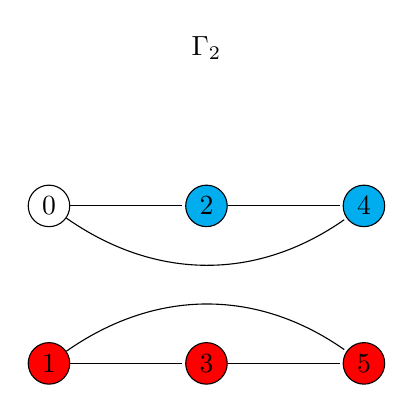
\begin{tikzpicture}[shorten >=1pt,auto,node distance=2cm,
				thin,main node/.style = {circle,draw, inner sep = 0pt, minimum size = 15pt}]	
				\node[main node,fill=white] (1) {0};
				\node[main node,fill=cyan] [right of = 1](2) {2};
				\node[main node,fill=cyan] [right of = 2](3) {4};
				\node[main node,fill=red] [below of = 1](4) {1};
				\node[main node,fill=red] [right of = 4](5) {3};
				\node[main node,fill=red] [right of = 5](6) {5};
				\node [above of =2] {$\Gamma_2$};
				
				\path[-]
				(1)edge node {} (2)
				edge [bend right=35] node {} (3)
				(2)edge node {} (3)
				(4)edge node {} (5)
				edge [bend left=35] node {} (6)
				(5) edge node {} (6);
				\end{tikzpicture}
				\end{aligned}$}\end{center}
		\caption[Graphs of $K_{3,3}$.]{The three graphs of $K_{3,3}$. The subconstituents of vertex $0$ are colored white, red,  and blue respectively.}\label{k33}
	\end{figure}
	The intersection numbers, Krein parameters, and eigenmatrices are
	\[\begin{aligned}L_0 &= \left[\begin{array}{cccc}
	1&0&0\\
	0&1&0\\
	0&0&1\\
	\end{array}\right],\quad L_1 &= \left[\begin{array}{cccc}
	0&3&0\\
	1&0&2\\
	0&3&0\\
	\end{array}\right],\quad L_2 &= \left[\begin{array}{cccc}
	0&0&2\\
	0&2&0\\
	1&0&1\\
	\end{array}\right];\\
	L_0^* &= \left[\begin{array}{cccc}
	1&0&0\\
	0&1&0\\
	0&0&1\\
	\end{array}\right],\quad L_1^* &= \left[\begin{array}{cccc}
	0&4&0\\
	1&2&1\\
	0&4&0\\
	\end{array}\right],\quad L_2^* &= \left[\begin{array}{cccc}
	0&0&1\\
	0&1&0\\
	1&0&0\\
	\end{array}\right];\end{aligned}\]
	\[P = \left[\begin{array}{rrr}
	1&3&2\\
	1&0&-1\\
	1&-3&2\\
	\end{array}\right],\qquad Q = \left[\begin{array}{rrr}
	1&4&1\\
	1&0&-1\\
	1&-2&1\\
	\end{array}\right].\]
	Now consider a second $2$-class association scheme given by the vertices of the octahedron, where the two nontrivial relations are defined as before. The three graphs for this scheme are
	\begin{figure}[H]\begin{center}\scalebox{.7}{$\begin{aligned}
				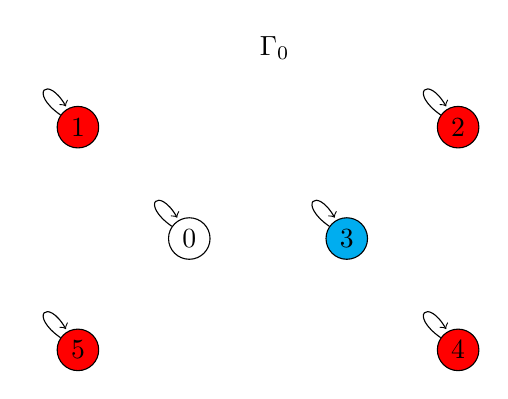
\begin{tikzpicture}[shorten >=1pt,auto,node distance=2cm,
				thin,main node/.style = {circle,draw, inner sep = 0pt, minimum size = 15pt}]
				
				\node[main node,fill=red] (2) {1};
				\node[main node,fill=white] [below right of = 2](1) {0};
				\node[main node,fill=cyan] [right of = 1](6) {3};
				\node[main node,fill=red] [above right of = 6](3) {2};
				\node[main node,fill=red] [below right of = 6](4) {4};
				\node[main node,fill=red] [below left of  = 1](5) {5};
				\node at (2.5,1) (9) {$\Gamma_0$};
				
				\path (1) edge [in=120,out=145,loop] ();
				\path (2) edge [in=120,out=145,loop] ();
				\path (3) edge [in=120,out=145,loop] ();
				\path (4) edge [in=120,out=145,loop] ();
				\path (5) edge [in=120,out=145,loop] ();
				\path (6) edge [in=120,out=145,loop] ();
				
				\end{tikzpicture}\qquad&\qquad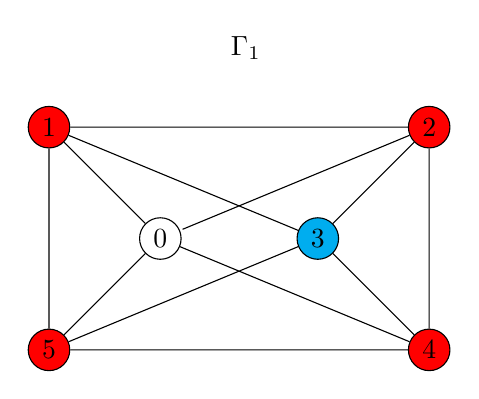
\begin{tikzpicture}[shorten >=1pt,auto,node distance=2cm,
				thin,main node/.style = {circle,draw, inner sep = 0pt, minimum size = 15pt}]
				
				\node[main node,fill=red] (2) {1};
				\node[main node,fill=white] [below right of = 2](1) {0};
				\node[main node,fill=cyan] [right of = 1](6) {3};
				\node[main node,fill=red] [above right of = 6](3) {2};
				\node[main node,fill=red] [below right of = 6](4) {4};
				\node[main node,fill=red] [below left of  = 1](5) {5};
				\node at (2.5,1) (9) {$\Gamma_1$};
				
				\draw[-] (1)--(2)--(3)--(4)--(5)--(2)--(6)--(5)--(1)--(4)--(6)--(3)--(1);
				\end{tikzpicture}\qquad\qquad
				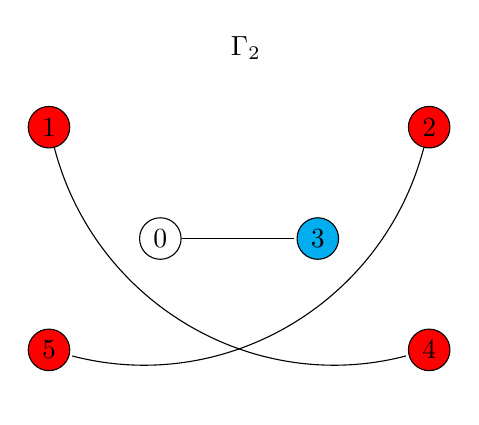
\begin{tikzpicture}[shorten >=1pt,auto,node distance=2cm,
				thin,main node/.style = {circle,draw, inner sep = 0pt, minimum size = 15pt}]	
				
				\node[main node,fill=red] (2) {1};
				\node[main node,fill=white] [below right of = 2](1) {0};
				\node[main node,fill=cyan] [right of = 1](6) {3};
				\node[main node,fill=red] [above right of = 6](3) {2};
				\node[main node,fill=red] [below right of = 6](4) {4};
				\node[main node,fill=red] [below left of  = 1](5) {5};
				\node at (2.5,1) (9) {$\Gamma_2$};
				
				\path[-]
				(1)edge node {} (6)
				(2)edge [bend right=45] node {} (4)
				(3)edge [bend left=45] node {} (5);
				\end{tikzpicture}
				\end{aligned}$}\end{center}
		\caption[Graphs of the octahedron.]{The three graphs of the octahedron. The subconstituents of vertex $0$ are colored white, red, and blue respectively.}\label{octahedron}
	\end{figure}
	The intersection numbers, Krein parameters, and eigenmatrices of this association scheme are
	\[\begin{aligned}
	L_0 &= \left[\begin{array}{cccc}
	1&0&0\\
	0&1&0\\
	0&0&1\\
	\end{array}\right],\quad L_1 &= \left[\begin{array}{cccc}
	0&4&0\\
	1&2&1\\
	0&4&0\\
	\end{array}\right],\quad L_2 &= \left[\begin{array}{cccc}
	0&0&1\\
	0&1&0\\
	1&0&0\\
	\end{array}\right];\\
	L_0^* &= \left[\begin{array}{cccc}
	1&0&0\\
	0&1&0\\
	0&0&1\\
	\end{array}\right],\quad L_1^* &= \left[\begin{array}{cccc}
	0&3&0\\
	1&0&2\\
	0&3&0\\
	\end{array}\right],\quad L_2^* &= \left[\begin{array}{cccc}
	0&0&2\\
	0&2&0\\
	1&0&1\\
	\end{array}\right];
	\end{aligned}\]
	\[P = \left[\begin{array}{rrr}
	1&4&1\\
	1&0&-1\\
	1&-2&1\\
	\end{array}\right],\qquad Q = \left[\begin{array}{rrr}
	1&3&2\\
	1&0&-1\\
	1&-3&2\\
	\end{array}\right].\]
	One may observe that the intersection numbers and the Krein parameters of the two schemes are interchanged, as well as the first and second eigenmatrices. This specific case is due to a duality arising from the context of \emph{translation schemes}\index{association schemes!translation schemes}: schemes for which there exists an abelian group $G$ acting regularly on the vertices with $(g(x),g(y))\in R_i$ if and only if $(x,y)\in R_i$ for every $x,y\in X$ and $g\in G$. When such a group exists, we may define a dual association scheme (also a translation scheme) $(\hat{X},\hat{\mathcal{R}})$ where $\hat{X} = \left\{\chi:\chi\in G^*\right\}$ and $(\chi,\chi')\in \hat{R}_i$ if and only if $E_i (\chi-\chi') = (\chi-\chi')$. In the case of the two association schemes given above, the desired group is $G\simeq \bbZ_6$ and we find each scheme results as the dual of the other. The pair of schemes listed is a specific case of the more general duality between $\overline{rK_s}$ and $\overline{sK_r}$; that is, the complement of $r$ copies of $K_s$ and the complement of $s$ copies of $K_r$ respectively. In this more general setting, we find that the cyclic group $\bbZ_{rs}$ acts regularly on each set of vertices.
	
	In general, we often find the automorphism group of an association scheme to be trivial; that is, there are no automorphisms of the vertices such that $(\pi(x),\pi(y))\in R_i$ if and only if $(x,y)\in R_i$ for every $0\leq i\leq d$ apart from the identity mapping. Therefore we do not expect to find a transitive action on the vertices, however we still find interesting properties when we strip away the group requirement and observe at the duality at the level of parameters. We say two association schemes are \emph{formally dual}\index{formal duality} if we may swap the eigenmatrices of one to get the eigenmatrices of the other (equivalently swapping the intersection numbers and Krein parameters of one gives the parameters of the other). In many cases, no dual scheme may exist; consider any association scheme for which the Krein parameters are not integral. This notion of formal duality still plays a major role in our understanding of the field of association schemes as a whole, motivating many of the questions we will focus on in this thesis. We finish this discussion with one final note: any definition based solely on the parameters of an association scheme will bring rise to analogous definitions for the dual. For instance, we find that $K_{3,3}$ is \emph{bipartite}\index{bipartite}, meaning $p^k_{ij}= 0$ whenever $i+j+k\notin2\bbZ$. The dual graph, the octahedron, must then have $q^k_{ij}=0$ whenever $i+j+k\notin2\bbZ$; we will call this \emph{dual-bipartite}\index{bipartite!dual-} or $Q$-bipartite (see \ref{poly}). Similarly, we find that both $K_{3,3}$ and the octahedron are \emph{antipodal graphs}\index{antipodal}: $p^d_{di} = 0$ whenever $i\notin\left\{0,d\right\}$. Both graphs are then what we call \emph{dual-antipodal}\index{antipodal!dual-} or $Q$-antipodal (see \ref{poly}): $q^d_{di}=0$ whenever $i\notin\left\{0,d\right\}$. While there has been much research into bipartite and antipodal graphs, in this thesis we are interested in the implications of these dual properties, seeking when such objects may exist and what structure they impose.
	\section{Feasibility and Realizability}
	One main point of interest is whether or not an association scheme exists, given a (possibly partial) parameter set. While existence often cannot be proven without explicitly constructing the scheme, we often may rule out the existence of a scheme due to the values its intersection numbers or Krein parameters must take. In this section we examine three main conditions which we will use throughout this thesis in addition to what we already stated in Lemma \ref{kitchensink}. We begin with an immediate restriction on the intersection numbers:
	\begin{lem}[\cite{Brouwer1989}]\label{intfeas}
		The intersection numbers of an association scheme must be non-negative integers.\qed
	\end{lem}
	This condition is easy to verify since, by definition, each $p^k_{ij}$ is the cardinality of a set. While this property is immediate, it can be a powerful tool to eliminate examples with very little information about the association scheme. Next consider the Krein parameters of our association scheme.
	\begin{lem}[\cite{Scott1973},Krein conditions]\label{kreinfeas}\index{Krein conditions}
		The Krein parameters of an association scheme must be non-negative real numbers.
	\end{lem}
	\begin{proof}
		From equation \eqref{Emult}, we find that $\nicefrac{q_{ij}^0}{\vert X\vert},\dots,\nicefrac{q_{ij}^d}{\vert X\vert}$ are the eigenvalues of $E_i\circ E_j$. However $E_i\circ E_j\in \BMA$ and therefore it must be symmetric, implying all of its eigenvalues are real. Further, $E_i\circ E_j$ is a principle submatrix of $E_i\otimes E_j$, which has two distinct eigenvalues: $1$ and $0$. Hence $E_i\otimes E_j$ is positive semidefinite and any principle submatrix must share the same property.
	\end{proof}
	The final feasibility condition we will list here is known as the \emph{absolute bound}\index{absolute bound}.
	\begin{lem}[\cite{Neumaier1981},Absolute bound]\label{absolute}
		The multiplicities $m_i$ ($0\leq i\leq d$) of a $d$-class association scheme satisfy:
		\[\sum_{q_{ij}^k\neq 0} m_k\leq\begin{cases}
		m_im_j & \text{ if }i\neq j\\
		\binom{m_i+1}{2} & \text{ if }i= j.
		\end{cases}\]
	\end{lem}
	\begin{proof}
		The sum on the left is the rank of $E_i\circ E_j$, a principle submatrix of the rank $m_im_j$ matrix $E_i\otimes E_j$. Further, if $i=j$, $E_i\circ E_j$ is the entrywise square of $E_i$. Assuming $\text{col}(E_i) = \text{span}(v_1,\dots,v_{m_i})$, the columns of $E_i\circ E_i$ must be linear combinations of the vectors $v_j\circ v_k$ for $1\leq j\leq k\leq d$, a total of $\binom{m_i+1}{2}$ vectors.
	\end{proof}
	There are many other feasibility conditions we may list here including some arising from design theory and others as simple as the handshaking lemma. In this thesis however, we are consider the conditions already stated to be a baseline for our to start with. Thus, we do not claim that any parameter set fulfilling these conditions is guaranteed to correspond to the parameters of some association scheme, rather we instead simply ignore parameter sets which do not fulfill these basic parameter restrictions. We therefore define two separate terms which will be used throughout this thesis, \emph{feasible paramter sets}\index{feasible parameter set} and \emph{realizable parameter sets}\index{realizable parameter set}. 
	\begin{definition}
		A \emph{feasible parameter set} is a set of Krein parameters, intersection numbers, and eigenmatrices such that:
		\begin{itemize}
			\item[FC1:] The Krein parameters satisfy Lemmas \ref{kreinfeas} and \ref{kitchensink} $(i')--(xiii')$,
			\item[FC2:] The intersection numbers satisfy Lemmas \ref{intfeas} and \ref{kitchensink} $(i)--(xiii)$,
			\item[FC3:] The integers $m_j = q^0_{jj}$ must satisfy Lemma \ref{absolute}.
		\end{itemize}
	\end{definition}
	\begin{definition}
		A feasible parameter set is \emph{realizable} if there exists an association scheme $(X,\cR)$ with the given parameter set.
	\end{definition}
	\section{Imprimitivity}\label{imprimitivity}
	In standard graph theory, one finds many ``products" which take two graphs and build larger graphs out of them. This notion of building larger objects from smaller ones is found in many other fields of mathematics including basic number theory where fundamental questions arise in identifying which numbers are ``prime". The field of association schemes is no exception; we often distinguish between those schemes which cannot be built from smaller schemes, calling them \emph{primitive}\index{imprimitivity!primitive}, and those which are ``products" of smaller schemes in a sense, referring to them as \emph{imprimitive}. More precisely, an association scheme $(X,\cR)$ is \emph{imprimitive} \index{imprimitivity!imprimitive}if there exists a non-trivial union of relations which results in an equivalence relation. When this occurs, we may break the scheme into two smaller schemes: the \emph{subscheme}\index{imprimitivity!subscheme} and the \emph{imprimitivity!quotient scheme}\index{imprimitivity!quotient scheme}; we define both in this section. We find that a scheme is imprimitive if and only if there exists a disconnected non-trivial relation. For instance, consider the association scheme $K_{3,3}$ depicted in Figure \ref{k33} and note that the union of relations $R_0\cup R_2$ create an equivalence relation with two equivalence classes. Whenever this occurs we call the set of relations which form the equivalence relation a \emph{system of imprimitivity}\index{imprimitivity!systems of -} and denote the set of corresponding indices by $\cI$. In some cases, we may have multiple systems of imprimitivity in our association scheme. For instance consider Example \ref{3cube} and note that $\cI_1 = \left\{0, 2\right\}$ and $\cI_2 = \left\{0, 3\right\}$ are both systems of imprimitivity yet $\cI_1$ admits two equivalence classes while $\cI_2$ admits four. Thus we must be careful to distinguish between distinct systems of imprimitivity for any given association scheme. In each case, we find that the size of any equivalence class is equal to the sum of the valencies corresponding to the indices in $\cI$; hence all classes have the same size for a given system of imprimitivity. In the example of the 3-cube, the size of each equivalence class for $\cI_1$ is $v_0+v_2 = 4$, likewise the size of each equivalence class for $\cI_2$ is $v_0+v_3 = 2$. For all that follows we denote the size of any given equivalence class by $r$ and then the number of equivalence classes by $w$ noting that $\vert X\vert = wr$. For each system of imprimitivity, we define two dual association schemes which arise: a subscheme and a quotient scheme. We note that the following derivation is non-standard as we will derive the schemes through their Bose-Mesner algebras. We do this to illuminate the duality at play, referring the reader to numerous other sources for a combinatorial derivation (\cite{Brouwer1989},\cite{Rao1984},\cite{Cameron1978},\cite{Martin2007}). 
	
	Suppose $(X,\cR)$ is given with the system of imprimitivity $\cI = \left\{0,i_1,\dots,i_s\right\}$ and equivalence classes $X_0,X_1,\dots,X_w$. Then $\left\{A_i\right\}_{i\in\cI}$ forms a basis for a second matrix algebra $\mathbb{B}\subset\BMA$ which is also closed under both matrix and Schur multiplication. We may order the vertices by equivalence classes so that every matrix in $\mathbb{B}$ is block diagonal with $w$ blocks of size $r\times r$. Further, \[\left[\sum_{i\in\cI}A_i\right]_{x,y} = \begin{cases}
	1 \text{ if there exists a }0\leq k\leq w\text{ with }x,y\in X_k,\\
	0 \text{ otherwise.}
	\end{cases}\]
	Thus $\sum_{i\in\cI}A_i = I_w\otimes J_r$ under this vertex ordering. As before, we find that $\mathbb{B}$ is commutative, and thus we may simultaneously diagonalize all matrices in $\mathbb{B}$ giving the basis of idempotents $\left\{E^\prime_i\right\}_{i\in\cI}$. Since our matrices are block diagonal with constant diagonal entries, the multiplicities of any eigenspace must be a multiple of $w$, the number of blocks on the diagonal. Then, since we have shown the rank $m$ matrix $I_w\otimes J_r\in\mathbb{B}$, we know that $\frac{1}{r}I_w\otimes J_r$ must be one of these matrices as it is has the minimum possible non-zero rank; call it $E^\prime_0$. As these idempotents correspond to the maximal common eigenspaces of $A_0,\dots,A_{i_s}$, every eigenspace of our original Bose-Mesner algebra must be contained within exactly one of these eigenspaces. Thus for $j\in\cI$ define $\hat{j} = \left\{i:E^\prime_j E_i = E_i\right\}$ and we must have $E_j^\prime = \sum_{b\in\hat{j}}E_b$. Therefore $\BMB$ is a second matrix algebra with an analogous pair of bases, idempotent under each operation. Due to the block structure, it becomes natural to instead consider this as $w$ distinct Bose-Mesner algebras on each equivalence class of vertices, noting that $I_r$ and $J_r$ are contained in each smaller algebra. In fact, one may check that the homomorphism $\psi_\ell$ mapping $A_i$ to the $\ell^\text{th}$ $r\times r$ diagonal block of $A_i$ is an algebra isomorphism from $\mathbb{B}$ to a Bose-Mesner algebra on $X_\ell$ preserving both products. The corresponding $s$-class association scheme $\left(X_\ell,\mathcal{R}^\prime\right)$ has relations given by $R_i^\prime = R_i\cap(X_\ell\times X_\ell) = \left.R_i\right\vert_{X_\ell}$ for $i\in\cI$; we call each such association scheme a \emph{subscheme}\index{imprimitivity!subscheme} of $(X,\cR)$. Since matrix multiplication is preserved by our mapping, we find that for $i,j,k\in\cI$, $p^{\prime k}_{ij} = p^k_{ij}$ and thus the intersection numbers match our original scheme for indices within $\cI$. While Schur products are also preserved by $\psi_\ell$, recall that the idempotents of $\mathbb{B}$ were not the same as the idempotents of our original scheme, thus we do not expect our Krein parameters to be preserved. Instead we must determine the parameters $q^{\prime k}_{ij}$ so that 
	\[E_i^\prime\circ E_j^\prime = \frac{1}{\vert X_\ell\vert} \sum_{k\in\cI}q^{\prime k}_{ij}E_k^\prime.\]
	First, note that such constants must exist since $\mathbb{B}$ is closed under entrywise multiplication. Now, recalling that $E_i^\prime = \sum_{a\in\hat{i}} E_a$, we may multiply each side of the above equation by $E_h$ for some $0\leq h\leq d$ and find
	\[\frac{1}{\vert X\vert}\sum_{a\in\hat{i},b\in\hat{j}} q^h_{ab}E_h = \left(E_i^\prime\circ E_j^\prime\right)E_h = \frac{1}{\vert X_\ell\vert}q^{\prime k}_{ij} E_h \]
	where $h\in\hat{k}$. Thus we find
	\begin{equation}q^{\prime k}_{ij} = \frac{1}{w}\sum_{a\in\hat{i},b\in\hat{j}}q^k_{ab}.\end{equation}
	 We note that, while the algebras of each subscheme must be isomorphic, the $w$ distinct subschemes need not be isomorphic; that is, there exists an algebra isomorphism $\psi_i\circ\psi_j^{-1}$ mapping $\BMA_j\rightarrow\BMA_i$, however there need not be an isomorphism mapping $X_j\rightarrow X_i$ for which $(\gamma(x),\gamma(y))\in R_i^\prime$ if and only if $(x,y)\in R_i^\prime$.
	
	We now consider the dual notion, the \emph{quotient scheme}\index{imprimitivity!quotient scheme}, by swapping the roles of our adjacency matrices and idempotents in the above derivation. First observe that Lemma \ref{kitchensink} $(i')$ applied to any subscheme tells us that $q^{\prime k}_{00} = 0$ for any $k\neq 0$. Thus, our original scheme must have $q^k_{ab} = 0$ whenever $a,b\in\hat{0}$ and $k\notin\hat{0}$. We denote $\cJ = \hat{0}$ and find that this implies the set of matrices $\left\{E_j\right\}_{j\in\cJ}$ is closed under entrywise multiplication. Therefore we have a third commutative matrix algebra $\mathbb{B}^\prime = \text{span}_{j\in\cJ}\left(E_j\right)$ closed under both matrix and Schur multiplication. Using the same argument as before, we note that $\mathbb{B}^\prime$ must be commutative with respect to the Schur product and therefore we may guarantee the existence of Schur idempotents (01-matrices) which span our matrix algebra. Let $\left\{A^\prime_j\right\}_{j\in\cJ}$ correspond to the set of minimal idempotents; that is, the idempotents contained in $\BMB^\prime$ which are not sums of other Schur idempotents in $\BMB^\prime$. These new idempotents correspond to the maximal common Schur-eigenspaces of $\mathbb{B}^\prime$ and, since $\mathbb{B}^\prime\subset\BMA$, we must have sets $\tilde{i} = \left\{j:A^\prime_i\circ A_j = A_j\right\}$ for $i\in\cJ$ giving $A^\prime_i = \sum_{j\in\tilde{i}}A_j$. Further, $\sum_{j\in\cJ} E_j = \frac{1}{r}I_{w}\otimes J_r$ and thus $I_{w}\otimes J_r\in\mathbb{B}^\prime$. This implies of the these Schur idempotents is $I_w\otimes J_r$; call it $A^\prime_0$, noting that therefore $\tilde{0} = \cI$. Using the set $\left\{E_j\right\}_{j\in \cJ}$ as a basis for $\BMB^\prime$, we find that $A^\prime_iA^\prime_0 = A^\prime_i\left(r\sum_{j\in \cJ} E_j\right) = rA^\prime_i$ and therefore we must have that each $A^\prime_i$ is a block matrix, constant on each block. Thus there exist symmetric matrices $\tilde{A}_i$ for $i\in\cJ$ such that $A^\prime_i = J_r\otimes \tilde{A}_i$ and we may define an algebra homomorphism $\tilde{\psi}$ mapping $A^\prime_i\mapsto \tilde{A}_i$ which preserves elementwise multiplication. We further find that
	\begin{equation}\tilde{\psi}\left(AB\right) = r\tilde{\psi}(A)\tilde{\psi}(B).\label{tildepsiprod}\end{equation}
	Then $\tilde{\psi}(A^\prime_0) = I$, $\tilde{\psi}\left(\sum_{i\in\cJ}A_i\right) =J_w$, and equation \eqref{tildepsiprod} gives us,
	\[\tilde{p}^{\tilde{k}}_{\tilde{i}\tilde{j}} = \frac{1}{r}\sum_{i\in\tilde{i},j\in\tilde{j}}p^k_{ij}\]
	for any choice of $k\in\tilde{k}$; this smaller algebra fulfills all the requirements of a Bose-Mesner algebra. Further, since $\tilde{\psi}$ preserves elementwise products, we find that $\tilde{q}^k_{ij} = q^k_{ij}$ for $i,j,k\in\cJ$. The resulting Bose-Mesner algebra is called the \emph{quotient scheme}\index{imprimitivity!quotient scheme}. Combinatorially, this is the association scheme $\left(\tilde{X},\tilde{\mathcal{R}}\right)$ where $\tilde{X}$ is the set of $w$ equivalence classes and $(X_i,X_j)\in \tilde{R}_{\tilde{i}}$ if there exists $x\in X_i$, $y\in X_j$, and $k\in \tilde{i}$ such that $(x,y)\in R_k$. 
	
	From the above two derivations we find that both the subscheme and the quotient scheme may be found by finding a subset of idempotents under one product which are closed under the second product. When this occurs we find a smaller matrix algebra which is isomorphic to a Bose-Mesner algebra on fewer vertices. Thus the main difference between a subscheme and a dual scheme is simply which set of idempotents we begin with (or rather, which product we take idempotents for). Throughout this thesis we will use $\tilde{i}$ to describe an index of the quotient scheme and $i^\prime$ an index of the subscheme. Further $\cI$ and $\cJ$ will continue to denote the subset of indices for which
	\[\sum_{i\in\cI} A_i = I_w\otimes J_r = r\sum_{j\in\cJ} E_j.\]
	In summary, we have the following theorem from \cite{Martin2007} as well as a lemma concerning the eigenmatrices of the subscheme and quotient scheme.
	\begin{thm}[\cite{Martin2007}] \label{mmw}The following are equivalent:
		\begin{enumerate}[label=(\roman*)]
			\item $(X,\mathbb{R})$ is imprimitive;
%			\item for some $j>0$, $E_j$ has repeated columns;
			\item for some subset $\mathcal{I} = \left\{i_0=0,i_1,\dots,i_s\right\}$ of $\left\{0,1,\dots,d\right\}$ and some ordering of the vertices $\sum_{h=0}^s A_{i_h} = I_w\otimes J_r$ for integers $w$ and $r$ with $\vert X\vert=wr$, $1<w,r<\vert X\vert$;
			\item for some subset $\mathcal{J} = \left\{j_0=0,j_1,\dots,j_s\right\}$ of $\left\{0,1,\dots,d\right\}$ and some ordering of the vertices $\sum_{h=0}^s E_{j_h} = \frac{1}{r}\left(I_w\otimes J_r\right)$ for integers $w$ and $r$ with $\vert X\vert=wr$, $1<w,r<\vert X\vert$.\qed
		\end{enumerate}
	\end{thm}
	\begin{lem}\label{repeatedcols}
	Let $P$ and $Q$ be the first and second eigenmatrix of an imprimitive association scheme with a system of imprimitivity given by $\cI$ and $\cJ$. Let $P^\prime$ be the first eigenmatrix of the subscheme and $\tilde{Q}$ be the second eigenmatrix of the quotient scheme. Then for any $i\in \cI$ and $j\in \cJ$ we have
	\[P^\prime_{\hat{k}i} = P_{ki},\qquad \tilde{Q}_{\tilde{k}j} = Q_{kj}\]
	where $\hat{k}$ is the relation in the subscheme which contains the image of $R_k$ and $\tilde{k}$ is the idempotent of the quotient scheme containing the image of $E_k$.\qed
	\end{lem}
	We finish this section by providing an illustration of each type of scheme, returning to the example of the $3$-cube. Recall that this association scheme had two systems of imprimitivity: $\cI_1 = \left\{0, 2\right\}$ and $\cI_2 = \left\{0, 3\right\}$. We begin with $\cI_1 = \left\{0,2\right\}$ and display the components of $\Gamma_2$ below.
		\begin{center}\scalebox{.7}{$\begin{aligned}
				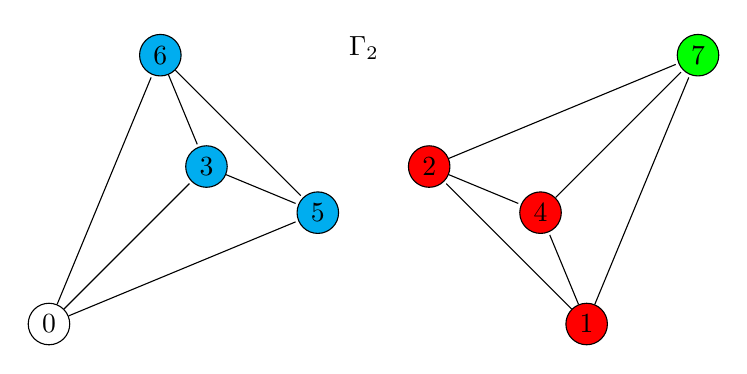
\begin{tikzpicture}[shorten >=1pt,auto,node distance=2cm,
				thin,main node/.style = {circle,draw, inner sep = 0pt, minimum size = 15pt}]
				
				\node[main node,fill=white] (1) {0};
				\node [right of = 1](2) {};
				\node [above of = 1](3) {};
				\node[main node,fill=cyan] [right of = 3](4) {3};
				\node [above right of = 1](5) {};
				\node[main node,fill=cyan] [right of = 5](6) {5};
				\node[main node,fill=cyan] [above of = 5] (7) {6};
				\node [right of = 7](8) {};
				
				\node [below right of =6] (11) {};
				\node[main node,fill=red] [right of = 11](12) {1};
				\node[main node,fill=red] [above of = 11](13) {2};
				\node [right of = 13](14) {};
				\node[main node,fill=red] [above right of = 11](15) {4};
				\node [right of = 15](16) {};
				\node [above of = 15] (17) {};
				\node[main node,fill=green] [right of = 17](18) {7};
				\node at (4,3.5) (9) {$\Gamma_2$};
				
				\path[-]
				(1)edge node {} (4)
				edge node {} (6)
				edge node {} (7)
				(12)edge node {} (13)
				edge node {} (15)
				edge node {} (18)
				(13)edge node {} (15)
				edge node {} (18)
				(4) edge node {} (6)
				(7) edge node {} (4)
				edge node {} (6)
				(15) edge node {} (18);
				\end{tikzpicture}
				\end{aligned}$}\end{center}
			For each of the two components we find a subscheme isomorphic to $K_4$.
		\begin{center}\scalebox{.7}{$\begin{aligned}
				\begin{tikzpicture}[shorten >=1pt,auto,node distance=2cm,
				thin,main node/.style = {circle,draw, inner sep = 0pt, minimum size = 15pt}]
				
				\node[main node,fill=white] (1) {0};
				\node[main node,fill=cyan] [right of = 3](4) {1};
				\node[main node,fill=cyan] [right of = 5](6) {2};
				\node[main node,fill=cyan] [above of = 5] (7) {3};
				\node at (2,4.5) (9) {$\Gamma_0^\prime$};
				
				\path (1) edge [in=120,out=145,loop] ();
				\path (4) edge [in=120,out=145,loop] ();
				\path (6) edge [in=120,out=145,loop] ();
				\path (7) edge [in=120,out=145,loop] ();
				
				\end{tikzpicture}\qquad\qquad
				\begin{tikzpicture}[shorten >=1pt,auto,node distance=2cm,
				thin,main node/.style = {circle,draw, inner sep = 0pt, minimum size = 15pt}]
				
				\node[main node,fill=white] (1) {0};
				\node[main node,fill=cyan] [right of = 3](4) {1};
				\node[main node,fill=cyan] [right of = 5](6) {2};
				\node[main node,fill=cyan] [above of = 5] (7) {3};
				\node at (2,4.5) (9) {$\Gamma_1^\prime$};
				
				\path[-]
				(1)edge node {} (4)
				edge node {} (6)
				edge node {} (7)
				(4) edge node {} (6)
				(7) edge node {} (4)
				edge node {} (6);
				\end{tikzpicture}
				\end{aligned}$}\end{center}
			The quotient scheme is found by collapsing each component to a single point, giving an association scheme isomorphic to $K_2$.
			\begin{center}\scalebox{.7}{$\begin{aligned}
			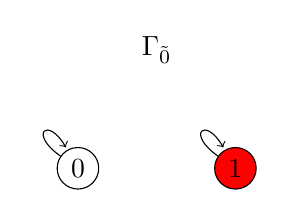
\begin{tikzpicture}[shorten >=1pt,auto,node distance=2cm,
			thin,main node/.style = {circle,draw, inner sep = 0pt, minimum size = 15pt}]
			
			\node[main node,fill=white] (1) {0};
			\node[main node,fill=red] [right of = 1](2) {1};
			\node at (1,1.5) (9) {$\Gamma_{\tilde{0}}$};
			
			\path (1) edge [in=120,out=145,loop] ();
			\path (2) edge [in=120,out=145,loop] ();
			
			\end{tikzpicture}\qquad\qquad
			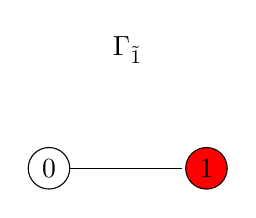
\begin{tikzpicture}[shorten >=1pt,auto,node distance=2cm,
			thin,main node/.style = {circle,draw, inner sep = 0pt, minimum size = 15pt}]
			
			\node[main node,fill=white] (1) {0};
			\node[main node,fill=red] [right of = 1](2) {1};
			\node at (1,1.5) (9) {$\Gamma_{\tilde{1}}$};
			
			\path[-]
			(1)edge node {} (2);
			\end{tikzpicture}
		\end{aligned}$}\end{center}
	Similarly, the system of imprimitivity given by $\cI_2 = \left\{0,3\right\}$ results in the following components of $\Gamma_3$:
	\begin{center}\scalebox{.7}{$\begin{aligned}
			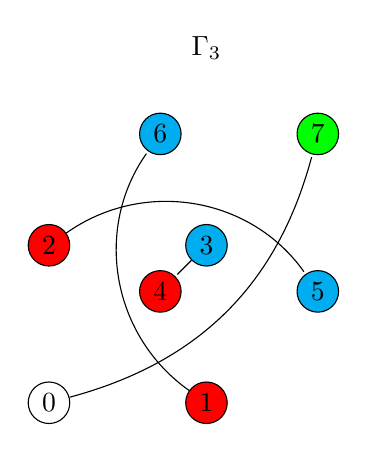
\begin{tikzpicture}[shorten >=1pt,auto,node distance=2cm,
			thin,main node/.style = {circle,draw, inner sep = 0pt, minimum size = 15pt}]
			
			\node[main node,fill=white] (1) {0};
			\node[main node,fill=red] [right of = 1](2) {1};
			\node[main node,fill=red] [above of = 1](3) {2};
			\node[main node,fill=cyan] [right of = 3](4) {3};
			\node[main node,fill=red] [above right of = 1](5) {4};
			\node[main node,fill=cyan] [right of = 5](6) {5};
			\node[main node,fill=cyan] [above of = 5] (7) {6};
			\node[main node,fill=green] [right of = 7](8) {7};
			\node at (2,4.5) (9) {$\Gamma_3$};
			
			\path[-]
			(1) edge [bend right] node {} (8)
			(2) edge [bend left=45] node {} (7)
			(3) edge [bend left=45] node {} (6)
			(4) edge node {} (5);
			\end{tikzpicture}
			\end{aligned}$}\end{center}
		Each component here results in a subscheme isomorphic to $K_2$,
		\begin{center}\scalebox{.7}{$\begin{aligned}
				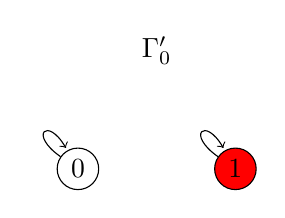
\begin{tikzpicture}[shorten >=1pt,auto,node distance=2cm,
				thin,main node/.style = {circle,draw, inner sep = 0pt, minimum size = 15pt}]
				
				\node[main node,fill=white] (1) {0};
				\node[main node,fill=red] [right of = 1](2) {1};
				\node at (1,1.5) (9) {$\Gamma_0^\prime$};
				
				\path (1) edge [in=120,out=145,loop] ();
				\path (2) edge [in=120,out=145,loop] ();
				
				\end{tikzpicture}\qquad\qquad
				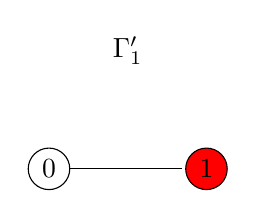
\begin{tikzpicture}[shorten >=1pt,auto,node distance=2cm,
				thin,main node/.style = {circle,draw, inner sep = 0pt, minimum size = 15pt}]
				
				\node[main node,fill=white] (1) {0};
				\node[main node,fill=red] [right of = 1](2) {1};
				\node at (1,1.5) (9) {$\Gamma_1^\prime$};
				
				\path[-]
				(1)edge node {} (2);
				\end{tikzpicture}
				\end{aligned}$}\end{center}
			while, the quotient scheme is isomorphic to $K_4$.
			
			\begin{center}\scalebox{.7}{$\begin{aligned}
					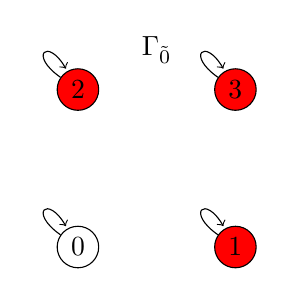
\begin{tikzpicture}[shorten >=1pt,auto,node distance=2cm,
					thin,main node/.style = {circle,draw, inner sep = 0pt, minimum size = 15pt}]
					
					\node[main node,fill=white] (1) {0};
					\node[main node,fill=red] [right of = 1](2) {1};
					\node[main node,fill=red] [above of = 1](3) {2};
					\node[main node,fill=red] [above of =2](4) {3};
					\node at (1,2.5) (9) {$\Gamma_{\tilde{0}}$};
					
					\path (1) edge [in=120,out=145,loop] ();
					\path (2) edge [in=120,out=145,loop] ();
					\path (3) edge [in=120,out=145,loop] ();
					\path (4) edge [in=120,out=145,loop] ();
					
					\end{tikzpicture}\qquad&\qquad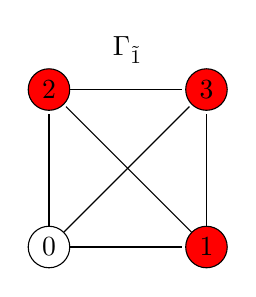
\begin{tikzpicture}[shorten >=1pt,auto,node distance=2cm,
					thin,main node/.style = {circle,draw, inner sep = 0pt, minimum size = 15pt}]
					
					\node[main node,fill=white] (1) {0};
					\node[main node,fill=red] [right of = 1](2) {1};
					\node[main node,fill=red] [above of = 1](3) {2};
					\node[main node,fill=red] [above of =2](4) {3};
					\node at (1,2.5) (9) {$\Gamma_{\tilde{1}}$};
					
					\path[-]
					(1) edge node {} (2)
					edge node {} (3)
					edge node {} (4)
					(2) edge node {} (3)
					edge node {} (4)
					(3) edge node {} (4);
					\end{tikzpicture}
					\end{aligned}$}\end{center}
	\section{Polynomial schemes}\label{poly}
	In this section we define and develop the notion of polynomial association schemes. We again present two dual concepts, $P$-polynomial and $Q$-polynomial, though we will focus primarily on the $Q$-polynomial case outside of this section. Let $(X,\cR)$ be a $d$-class association scheme. We say $(X,\cR)$ is \emph{$Q$-polynomial}\index{$Q$-polynomial}, or \emph{cometric}\index{$Q$-polynomial!cometric}, if there exists an ordering of the idempotents, say $E_0,E_1,\dots,E_d$, such that the Krein parameters satisfy the following conditions:
	\begin{enumerate}
		\item $q^k_{ij} = 0$ whenever $k>i+j$, and
		\item $q^k_{ij} > 0$ whenever $k = i+j$.
	\end{enumerate}
	Additionally, we note that it is sufficient to check only the above conditions with $i=1$ (see \cite[Prop.\ 2.7.1]{Brouwer1989}). Thus we may characterize $Q$-polynomial association schemes as exactly those for which there exists an eigenspace ordering for which the Krein array ($L_1^*$) is irreducible tridiagonal. When this occurs, we find that $\BMA = \left<E_1\right>_\circ$; that is, $E_1$ generates our entire Bose-Mesner algebra using Schur products. Additionally, for each $0\leq k\leq d$, we may define a single variable polynomial $q_k(t)$ of degree $k$ so that $Q_{ik} = q_k\left(Q_{i1}\right)$ for $0\leq i\leq d$. This is equivalent to $E_k = \frac{1}{\vert X\vert}q_k\circ\left(\vert X\vert E_1\right)$; that is $q_k$ applied entrywise to $\vert X\vert E_1$ results in $\vert X\vert E_k$ (again see \cite[Prop.\ 2.7.1]{Brouwer1989}). Then we may define one final polynomial $q_{d+1}(t)$ with degree $d+1$ such that $q_{d+1}\circ(\vert X\vert E_1) = 0$. This immediately implies that $E_1$ has $d+1$ distinct entries and we find it convenient to order the relations according to these values so that $Q_{01}>Q_{11}>\dots>Q_{d1}$; we call this the \emph{natural ordering}\index{natural ordering} with respect to the $Q$-polynomial ordering $E_0,E_1,\dots,E_d$. As is suggested by this definition, it is possible to find multiple $Q$-polynomial orderings for the same association scheme. However, Suzuki showed (\cite{Suzuki1998-2}) that, with the exception of cycles, any $Q$-polynomial association scheme has at most two $Q$-polynomial orderings. We say a $Q$-polynomial association scheme is \emph{$Q$-bipartite}\index{$Q$-polynomial!$Q$-bipartite} if the Krein parameters fulfill the additional requirement $q^k_{ij} = 0$ whenever $i+j+k\notin 2\bbZ$. We find in this case that $\left\{E_i\right\}_{i\in 2\bbZ}$ serves as a Schur-closed subalgebra. Additionally we say a $Q$-polynomial scheme is \emph{$Q$-antipodal}\index{$Q$-polynomial!$Q$-antipodal} if $q^k_{dd} = 0$ whenever $k\notin\left\{0,d\right\}$ and thus $\left\{E_0,E_d\right\}$ is a Schur-closed subalgebra. Each case results in a system of imprimitivity; the following is Suzuki's theorem concerning these systems of imprimitivity.
	\begin{thm}[\cite{Suzuki1998},\cite{Cerzo2009},\cite{Tanaka2011}] \label{suzukiimprim} Suppose $(X,\mathcal{R})$ is an imprimitive cometric association scheme with $Q$-polynomial ordering $E_0,\dots,E_d$ and natural ordering $A_0,\dots,A_d$. Then one of the following holds:
	\begin{enumerate}[label=(\roman*)]
		\item $(X,\mathcal{R})$ is $Q$-bipartite and $\mathcal{J} = \left\{0,2,4,\dots\right\}$, $\mathcal{I} = \left\{0,d\right\}$;
		\item $(X,\mathcal{R})$ is $Q$-antipodal and $\mathcal{J} = \left\{0,d\right\}$, $\mathcal{I} = \left\{0,2,4,\dots\right\}$.
	\end{enumerate}
	\end{thm}
	The original theorem in \cite{Suzuki1998} allowed for two exceptional cases, one with $d=4$ and another with $d=6$. These two cases were later ruled out in \cite{Cerzo2009} and \cite{Tanaka2011} respectively.
	
	We now consider the dual notion: $P$-polynomial association schemes. Again let $(X,\cR)$ be a $d$-class association scheme. We say $(X,\cR)$ is \emph{$P$-polynomial}\index{$P$-polynomial}, or \emph{metric}\index{$P$-polynomial!metric}, if there exists an ordering of the relations, say $A_0,A_1,\dots,A_d$, such that the intersection numbers satisfy the following conditions:
	\begin{enumerate}
		\item $p^k_{ij} = 0$ whenever $k>i+j$, and
		\item $p^k_{ij} > 0$ whenever $k = i+j$.
	\end{enumerate}
	As before we find that it is sufficient to check the above conditions only when $i=1$ (\cite[Prop.\ 2.7.1]{Brouwer1989}) and thus an association scheme is $P$-polynomial if and only if there exists an ordering of the relations for which the intersection array $(L_1)$ is irreducible tridiagonal. In this case we find that $\BMA= \left<A_1\right>_*$ and it is therefore common to consider a $P$-polynomial scheme synonymous with $\Gamma_1$---a \emph{distance regular graph}; that is $(x,y)\in R_i$ if and only if $d_\Gamma(x,y) = i$. We find analogous results as we saw in the $Q$-polynomial case with \cite[Theorem 4.2.12]{Brouwer1989} and \cite{Taylor1978} giving that any $P$-polynomial association scheme which is not a cycle has at most two $P$-polynomial orderings. Further, we may define \emph{$P$-bipartite}\index{$P$-polynomial!bipartite} (or more commonly \emph{bipartite}) and \emph{$P$-antipodal}\index{$P$-polynomial!antipodal} (\emph{antipodal}) as those schemes for which $p^k_{ij}= 0$ if $i+j+k\not\in 2\bbZ$ and $p^k_{dd}= 0$ whenever $k\not\in\left\{0,d\right\}$ respectively. For these schemes we again find systems of imprimitivity. This time, however, $\mathcal{I} = \left\{0,2,4,\dots\right\}$ and $\mathcal{J} = \left\{0,d\right\}$ correspond to the bipartite scheme while $\mathcal{I} = \left\{0,d\right\}$ and $\mathcal{J} = \left\{0,2,4,\dots\right\}$ for the antipodal scheme. As before we find that these systems of imprimitivity are all that can occur for $P$-polynomial schemes (\cite{Smith1971},\cite{Gardiner1980}).
	
	Despite the close connection between $P$-polynomial and $Q$-polynomial association schemes, we note that many of the theorems mentioned here in the $P$-polynomial case predate their $Q$-polynomial analogues by as much as 30 years. Further, there are many other theorems which are known to be true for metric schemes whose $Q$ analogues have yet to be proven. For instance Taylor and Levingston showed in 1978 (\cite{Taylor1978}) that the sequence $k_0,k_1,\dots,k_d$ is unimodal, however the $Q$-analogue (the sequence $m_0,m_1,\dots,m_d$ is unimodal) remains a conjecture to this day. Chapter 6 of \cite{Brouwer1989} details the known examples of distance regular graphs at that time--all tables mentioned here appear in that chapter. Here they list 21 classical parameter sets (Tables 6.1 \& 6.2), 15 of which correspond to infinite families, three folded classical graphs (Table 6.3), nine near regular polygons including the generalized polygons (Tables 6.5 \& 6.6), as well as 20 more primitive distance regular graphs (Tables 6.8 \& 6.9). Further they give the known bipartite and antipodal examples (Tables 6.9 \& 6.10 resp.). On the $Q$-polynomial side however, \cite{Martin2007} lists the $Q$-polynomial association schemes known in 2007: those that are also $P$-polynomial as well as four infinite families and 22 sporadic examples. Concerning the association schemes which are both metric and cometric, we note the following conjecture of Bannai and Ito.
	\begin{conj*}[Bannai \& Ito] 
		For $d$ sufficiently large, a primitive association scheme with $d$ classes is metric if and only if it is cometric.
	\end{conj*}
	With this conjecture in mind, we expect that as $d$ grows, the fraction of $Q$-polynomial schemes which are not also $P$-polynomial should diminish. However, as can be seen by the tables hosted by Williford \cite{Willifordtable}, there is still much work to be done for small $d$. Note every primitive $2$-class association scheme (connected strongly regular graph) is both metric and cometric, thus we will primarily focus on schemes which are have at least three classes.
\section{PSD Cone}
\chapter{Positive semi-definite cone of an association scheme}\label{psdcone}
Consider the following classic unsolved problem in discrete geometry (\cite{Haantjes1948},\cite{vanLint1966},\cite{Lemmens1973}): Given a fixed positive integer $n$, what is the maximum number of lines through the origin one may find in $\mathbb{R}^n$ such that the angle between any pair of distinct lines is $\theta$. Over the past 70 years, researchers in both math and physics have developed the theory of these ``equiangular lines" (also ``equiangular tight frames"), finding upper bounds on the number of lines in any given dimension coming from tools such as linear programming \cite{Delsarte1975}, number theory \cite{Lemmens1973}, and more recently semi-definite programming \cite{Barg2014}. A related problem asks the question: How many orthonormal basis may we find in $\mathbb{R}^n$ such that the angle between vectors in distinct bases is fixed, called ``mutually unbiased bases" (see \cite{Delsarte1975}, \cite{Calderbank1997},\cite{Boykin2005}). While the complex analogue of both of these questions have had great interest in Quantum computing (\cite{Appleby2005},\cite{Grassl2008},\cite{Ivanovic1981},\cite{Wootters1989}), we restrict ourselves to the real cases in this document as our matrix algebras are all real.

Both of the problems mentioned above are restricted versions of the more general question of finding spherical $t$-distance sets: sets of unit vectors in a fixed dimension with only $t$ distinct inner products arising between distinct vectors. In each case we may recast the problem to looking for large positive semi-definite matrices with a low rank, constant diagonal, and few distinct entries off the diagonal. More precisely, let $G$ be a $n\times n$ positive semi-definite matrix with rank $r$. Then we may find a $d\times n$ matrix $U$ such that $G = U^TU$; that is $G$ is the Gram matrix of the columns of $U$. If $G$ has a constant diagonal, then we may scale the columns of $U$ so that each column is a unit vector. Then the set of columns of $U$ gives a spherical $t$-distance set where $t$ is the number of unique entries off the diagonal of $G$. Now recall that a $d$-class association scheme results in a Bose-Mesner algebra which $d+1$ basis idempotents. These idempotents serve as the basis of the cone of positive semi-definite matrices inside our Bose-Mesner algebra. In this chapter we will examine this cone and display how we may build large spherical $t$-distance sets by taking linear combinations of subsets of the idempotents. We will build examples of equiangular lines meeting the maximum possible number of lines in the given dimensions, as well as provide a method for determining which sets of equiangular lines may be derived from a given scheme. Finally, we will introduce a second positive definite cone and use a result of Sch\"{o}nberg to prove this cone must be contained within our original cone. This results in new constraints on general association schemes which we will examine further in the Cometric case.
\section{Cone of idempotents}
Let $(X,\cR)$ be an association scheme with basis relations $A_0,\dots,A_d$ and orthogonal idempotents $E_0,\dots,E_d$. Since each $E_i$ is an idempotent matrix, it has spectrum $\left\{0,1\right\}$ and thus is positive semi-definite, denoted $E_i\succeq 0$. Further, let 
\begin{equation}G = \sum_i\alpha_i E_i.\label{lincomb}\end{equation}
Then we have $\text{spec}\left(G\right) = \left\{\alpha_0,\dots,\alpha_d\right\}$. Therefore $G\succeq 0$ if and only if $\alpha_i\geq 0$ for all $0\leq i\leq d$. Thus the \emph{positive semi-definite cone} of $(X,\cR)$ is the set of non-negative linear combinations of the idempotents $E_0,\dots,E_d$. Further, equation \eqref{lincomb} gives us that \begin{equation}\text{rank}\left(G\right) = \sum_{\alpha_i\neq 0} m_i.\label{rank}\end{equation}
Finally, since $G\in\BMA$ we must have $G = \sum_i \beta_i A_i$ and thus there are at most $d$ unique values off the main diagonal, making $\frac{1}{\beta_0}G$ the Gram matrix of a spherical $t$ distance set where $t\leq d$. In Chapter $\ref{3class}$ we examine one type of cometric association scheme where the first idempotent, $E_1$, gives an interesting 3-distance set where, in the optimal case, the number of vectors scales as $\frac{1}{2}v^2$ for dimension $v$. In this same case we show that adding another idempotent, namely $E_0$, allows us to build large sets of real mutually unbiased bases by choosing $\alpha_0$ and $\alpha_1$ carefully so that the non-zero entries off the diagonal of $G$ have a constant modulus. Before moving to two examples coming from $3$-class primitive cometric association schemes, we note the following bound on the maximum number of equiangular lines in a given dimension known as the relative bound.
\begin{thm}[\cite{vanLint1966}]\label{relbound}
	Let $v_\alpha(n)$ be the maximum number of equiangular lines with inner products $\pm\alpha$ in $\mathbb{R}^n$. If $n<\alpha^{-2}$ then
	\[v_\alpha(n)\leq\frac{r(1-\alpha^2)}{1-r\alpha^2}.\]
\end{thm}
We now examine two 3-class primitive association schemes to illustrate how we may build equiangular lines from these schemes. We note that in both cases the system of lines is extremal with respect to the given angle, however there are other angles where the upper bound is much higher. The first we will consider comes from the Halved 7-cube while the second corresponds to the Dual Polar space $B_3(2)$.
\begin{example}
	Consider the 3-class primitive association scheme given by the Halved 7-cube \cite{Brouwer1989}. This scheme is both metric and cometric with the following eigenmatrices
	\[P = \left[\begin{array}{cccc}
	1& 21& 35& 7\\
	1& 9& -5& -5\\
	1& 1& -5& 3\\
	1& -3& 3& -1\\
	\end{array}\right],\qquad  Q= \left[\begin{array}{cccc}
	1& 7& 21& 35\\
	1& 3& 1& -5\\
	1& -1& -3& 3\\
	1& -5& 9& -5\\
	\end{array}\right].\]
	Recall that $E_j = \frac{1}{\vert X\vert}\sum_{i}Q_{ji}A_i$ and consider
	\[G = 16\left(E_1 + E_2\right).\]
	We may then use the entries of $Q$ to replace each idempotent with the corresponding sum of adjacency matrices giving 
	\[G = 7A_0 + A_1 -A_2+A_3.\]
	Then $\frac{1}{7}G$ is the Gram matrix of $64$ lines in dimension $m_1+m_2 = 28$ with inner product $\frac{1}{7}$. Using the relative bound, we find that this is the optimal number of equiangular lines possible in dimension $28$ with an inner product of $\frac{1}{7}$.
\end{example}
\begin{example}
	Consider the 3-class primitive cometric (and metric) association scheme known as the dual polar space $B_3(2)$. The first and second eigenmatrices are
	\[P = \left[\begin{array}{cccc}
	1& 14& 56& 64\\
	1& 5& -2& -8\\
	1& -1& -4& 4\\
	1& -7& 14& -8\\
	\end{array}\right],\qquad  Q= \left[\begin{array}{cccc}
	1& 35& 84& 15\\
	1& \nicefrac{25}{2}& -6& -\nicefrac{15}{2}\\
	1& -\nicefrac{5}{4}& -6& \nicefrac{15}{4}\\
	1& -\nicefrac{35}{8}& \nicefrac{21}{4}& -\nicefrac{15}{8}\\
	\end{array}\right].\]
	Consider the matrix
	\[G = \frac{1}{45}\left(5E_0+8E_1 + 8E_2\right) = 9A_0 + A_1 +A_2-A_3.\]
	Similar to before, $\frac{1}{9}G$ is the Gram matrix of $135$ lines in dimension $m_0+m_1+m_2 = 51$ with inner product $\frac{1}{9}$. Here, the relative bound tells us that optimal number of lines in dimension 51 with inner product $\frac{1}{9}$ is 136, thus this construction is within one line of being optimal.
\end{example}
\begin{comment}
\begin{example}
	Consider the 3-class primitive cometric association scheme coming from the Dual Kasami codes \cite{deCaen1999}. The first and second eigenmatrices are:
	\[P = \left[\begin{array}{cccc}
	1& 310& 527& 186\\
	1& 70& -17& -17\\
	1& 6& -17& 15\\
	1& -10& 15& -17\\
	\end{array}\right]\qquad  Q= \left[\begin{array}{cccc}
	1& 31& 465& 527\\
	1& 7& 9& -17\\
	1& -1& -15& 15\\
	1& -9& 25& -17\\
	\end{array}\right].\]
	Consider the matrix
	\[G = \frac{1024}{496}\left(E_1 + E_2\right) = A_0 + \frac{1}{31}A_1 -\frac{1}{31}A_2+\frac{1}{31}A_3.\]
	Similar to before, $G$ is the Gram matrix of $1024$ lines in dimension $m_1+m_2 = 496$ with inner product $\frac{1}{31}$. Using the relative bound, we find that this is the optimal number of equiangular lines possible in dimension $496$ with an inner product of $\frac{1}{31}$.
\end{example}
\end{comment}
In both of the examples above, we find linear combinations of the idempotents where the idempotent with largest multiplicity has coefficient 0. While we may allow ourselves to include this idempotent, doing so often results in line-sets which are far from optimal. Let us consider the case in general.

\begin{lem}\label{equilines}
Let $(X,\cR)$ be a $d$-class association scheme with second eigenmatrix $Q$ and idempotents $E_0,E_1,\dots,E_d$ with multiplicities $m_0,m_1,\dots,m_d$. Let $Q^\prime$ be the $d\times (d+1)$ submatrix of $Q$ given by deleting row $0$. Let $y\in\mathbb{R}^d$ be any of the $2^d$ vectors with each entry given by $\pm 1$ and let $x$ be a solution of $Q^\prime x = y$ (if one exists). If $x$ contains no negative entries then
\[G = \sum_{j=0}^dx_jE_j\]
is the Gram matrix of $\vert X\vert$ equiangular lines in dimension $\displaystyle{\sum_{x_j\neq 0} m_j}$ where the inner product between any two vectors has modulus $\left(\displaystyle{\sum x_jm_j}\right)^{-1}$.
\end{lem}
\begin{proof}
	Noting that $Q^\prime x = y$ we have the $d$ equations
	\[Q_{i1}x_1 + \dots + Q_{id}x_d = c_i\]
	for $1\leq i\leq d$ where each $c_i$ is either $1$ or $-1$.	Then
	\[G = \sum_{j\neq i}x_jE_j = \frac{1}{\vert X\vert}\sum_{i=0}^{d}\left(\sum_{j=0}^dQ_{ij}A_i\right) = \frac{1}{\vert X\vert}\sum_{j=0}^d x_jm_jA_0 + \frac{1}{\vert X\vert}\sum_{i=1}^d c_iA_i.\]
	Since $\vert c_i\vert = 1$ for each $1\leq i\leq d$, each off diagonal entry of $G$ has the same absolute value. Thus we may scale $G$ by its diagonal entry to obtain the Gram matrix of a set of equiangular unit vectors. Then the rank of $G$ is given by the sum of the ranks of each $E_j$ included in the sum and the inner product between pairs of unit vectors is the coefficient of $A_0$.
\end{proof}
The following results may be observed applying Lemma \ref{equilines} to the tables in \cite{Willifordtable}.
\begin{table}
	\begin{center}
	Optimal constructions\\
\begin{tabular}{l|c|c|ccl|c|c|c}
	Label & $\vert X\vert$ & $n$ & $\nicefrac{1}{\alpha}$&&Label & $\vert X\vert$ & $n$ & $\nicefrac{1}{\alpha}$ \\\cline{1-4}\cline{6-9}
$\left<64,7\right>^*$ & 64 & 28 & 7 & \qquad &$\left<1200,55\right>$ & 1200 & 110 & 11	\\ 
$\left<64,9\right>^*$ & 64 & 36 & 9 & \qquad	&$\left<1200,109a\right>$ & 1200 & 110 & 11\\
$\left<64,21\right>^*$ & 64 & 28 & 7 & \qquad &$\left<1344,79\right>$ & 1344 & 238 & 17 \\
$\left<120,9\right>^*$ & 120 & 35 & 7 & \qquad &$\left<1456,90a\right>$ & 1456 & 195 & 15 \\
$\left<120,14\right>^*$ & 120 & 35 & 7 &	\qquad &$\left<1456,97\right>$ & 1456 & 195 & 15 \\
$\left<120,17a\right>^*$ & 120 & 35 & 7 &\qquad  &$\left<1520,49\right>$ & 1520 & 589 & 31 \\
$\left<280,27a\right>$ & 280 & 63 & 9 &\qquad   &$\left<1520,56\right>$ & 1520 & 589 & 31 \\
$\left<324,19a\right>$ & 324 & 171 & 19 &\qquad  &$\left<1596,55\right>$ & 1596 & 551 & 29\\
$\left<344,42\right>$ & 344 & 43 & 7 & \qquad &$\left<2016,65\right>$ & 2016 & 651 & 31\\
$\left<460,51\right>$ & 460 & 69 & 9 & \qquad &$\left<2160,119\right>$ & 2160 & 255 & 17\\
$\left<540,44\right>$ & 540 & 99 & 11 & \qquad &$\left<2500,51\right>$ & 2500 & 1225 & 49\\
$\left<540,49\right>$ & 540 & 99 & 11 & \qquad &$\left<2500,75\right>$ & 2500 & 1275 & 51 \\
$\left<936,51\right>$ & 936 & 221 & 17 & \qquad &$\left<2016,62a\right>$ & 2016 & 651 & 31 \\
$\left<936,51a\right>$ & 936 & 221 & 17 & \qquad &$\left<2160,119a\right>$ & 2160 & 255 & 17 \\
$\left<1024,31\right>^*$ & 1024 & 496 & 31 & \qquad &$\left<2160,119b\right>$ & 2160 & 255 & 17 \\
$\left<1024,33\right>$ & 1024 & 528 & 33 & \qquad &$\left<2500,51a\right>$ & 2500 & 1275 & 51 \\
$\left<1024,66\right>^*$ & 1024 & 528 & 33 & \qquad 
\end{tabular}\\\vspace{1cm}
Near Optimal constructions\\
\begin{tabular}{l|c|c|ccl|c|c|c}
	Label & $\vert X\vert$ & $n$ &  $\nicefrac{1}{\alpha}$&&Label & $\vert X\vert$ & $n$ & $\nicefrac{1}{\alpha}$\\\cline{1-4}\cline{6-9}
$\left<35,6\right>^*$ & 35 & 21 & 7 & \qquad &$\left<729,56\right>$ & 729 & 337 & 25\\
$\left<135,35\right>^*$ & 135 & 51 & 9 & \qquad &$\left<923,70\right>$ & 923 & 143 & 13 \\
$\left<279,30\right>$ & 279 & 63 & 9 & \qquad &$\left<1035,68\right>$ & 1035 & 185 & 15 \\
$\left<319,28\right>$ & 319 & 88 & 11 & \qquad &$\left<1349,70\right>$ & 1349 & 285 & 19 \\
$\left<377,28\right>$ & 377 & 117 & 13 & \qquad &$\left<1975,78\right>$ & 1975 & 475 & 25 \\
$\left<527,30\right>$ & 527 & 187 & 17 & \qquad &$\left<2159,126\right>$ & 2159 & 255 & 17 \\
$\left<527,30a\right>$ & 527 & 187 & 17 & \qquad &$\left<2759,88\right>$ & 2759 & 713 & 31 \\
\end{tabular}
\caption[Optimal and near-optimal constructions for equiangular lines using 3-class primitive cometric association schemes]{In these tables we give the sets of equiangular lines which may be built if the given parameter sets for 3-class primitive cometric association schemes are realizable. The first table contains the examples where the number of lines is optimal, while the second contains those which are within one line of optimality. Each parameter set is listed in Williford's online tables \cite{Willifordtable} using the designator in the far left column. For each set we list the number of lines $\vert X\vert$, dimension $n$, and the inverse of the inner product $\frac{1}{\alpha}$. The labels with stars correspond to realizable parameter sets.}
\end{center}
\end{table}

\section{Sch\"{o}nberg's Theorem}
\include{schoenbergs}
\section{3-class $Q$-antipodal: LSSDs}
\chapter{3-class $Q$-antipodal: LSSDs}\label{3class}
\section{4-class $Q$-bipartite: Double covers of SRGs}
\chapter{Antipodal double covers of regular graphs}
\label{4classbip}
\section{Intro -- Will be removed, only here as a marker}

\section{Projective doubles of regular graphs}

Let $\Gamma$ be an undirected graph on $v$ vertices. A \emph{projective double} of $\Gamma$ is an antipodal (spherical) $4$-distance set, say $L = \left\{\ell_1,\dots,\ell_{2v}\right\}$ with inner products $A = \left\{1,\alpha,0,-\alpha,-1\right\}$, such that there exists a mapping $\phi:L\rightarrow V\Gamma$ fulfilling
\begin{enumerate}[label=(\roman*)]
	\item $\phi(\ell_i) = \phi(\ell_j)$ if and only if $\left\vert\left<\ell_i,\ell_j\right>\right\vert = 1$,
	\item $\phi(\ell_i) \sim \phi(\ell_j)$ if and only if $\left\vert\left<\ell_i,\ell_j\right>\right\vert = \alpha$
\end{enumerate}
for $1\leq i,j\leq 2v$. Since the inner products are determined by a single parameter $\alpha$, we will often refer to $L$ as a projective double of $\Gamma$ with inner product $\alpha$. For vertices $v,w\in V\Gamma$, $(ii)$ implies $v\not\sim w$ if and only if $\ell_v\perp\ell_w$ for any $\ell_v\in\phi^{-1}(v)$ and $\ell_w\in\phi^{-1}(w)$. We are interested in which graphs permit a projective double however, without any further restrictions on $L$, the result is uninteresting.
\begin{prop}\label{dirnaive}
	For any non-empty simple graph $\Gamma$, there exists a projective double in $\mathbb{R}^{m}$ for some $m\leq \vert V\Gamma\vert$ with $\alpha = d^{-1}$ with $d$ the max degree of $\Gamma$.
\end{prop}
\begin{proof}
	Let $\Gamma = \Gamma(V,E)$ be given. Now orient every edge of $\Gamma$ and define $e_i^+,e_i^-\in V$ so that $e_i = (e_i^-,e_i^+)$, thus $e_i$ points from vertex $e_i^-$ to $e_i^+$. Let $M$ be the matrix with rows indexed by vertices and columns indexed by edges such that
	\[\left[M\right]_{ij} =\begin{cases} 1 &\text{ if }v_i = e_j^+\\
	-1 &\text{ if }v_i = e_j^-\\
	0 &\text{ otherwise. }
	\end{cases}\]
	Then we find 
	\[\left[MM^T\right]_{ij} = \begin{cases}
	k_i & \text{ if }i=j,\\
	1 & \text{ if } i\sim j,\\
	0 & \text{ otherwise}
	\end{cases}\]
	where $k_i$ is the degree of vertex $i$. Thus two distinct rows are orthogonal if and only if their corresponding vertices are non-adjacent. However unless $k_i$ is constant independent of $i$ (the graph is regular), the rows do not have the same norm. To solve this, let $d = \max_{i}(k_i)$ (the max degree of $\Gamma$) and define the diagonal matrix $D$ whose $i^\text{th}$ diagonal entry is $\sqrt{d-k_i}$. Then the matrix $N = \left[\begin{array}{c|c}
	M & D
	\end{array}\right]$ has the property that
	\[\left[NN^T\right]_{ij} = \left[MM^T\right]_{ij} + (k-k_i)\delta_{ij} = \begin{cases}
	d & \text{ if }i=j,\\
	1 & \text{ if } i\sim j,\\
	0 & \text{ otherwise.}
	\end{cases}\]
	Thus the rows of $\frac{1}{\sqrt{d}}N$, along with their negatives, result in a projective double of $\Gamma$ with inner product $\frac{1}{d}$. Further the rank of $N$ is no larger than $\max\left\{\vert V\vert, \vert V\vert+\vert E\vert\right\} = \vert V\vert$.
\end{proof}
\begin{cor}\label{regnaive}
	For any regular graph $\Gamma$ with regularity $k>0$, there exists a projective double in $\mathbb{R}^m$ with inner product $\frac{1}{k}$ for some $m\leq T$ where $T$ is the number of edges in any spanning forest.
\end{cor}
\begin{proof}
	We follow the same proof as with Proposition \ref{dirnaive}, however we note that since our graph is regular, the rows of $M$ all have the same norm. Thus the normalized rows (with their negatives) suffice as our projective double. Now, consider any cycle $C$ in $\Gamma$ and assume without loss of generality that $C = \left\{e_1,\dots,e_s\right\}$. Then, replacing a column with its negative if necessary, $\displaystyle{M_{e_s} = \sum_{i=1}^{s-1}M_{e_{i}}}$. We then reorder the columns of $M$ so that the first $T$ edges correspond to the edges of a spanning forest and note that every remaining column induces a linear dependence.
\end{proof}
Proposition \ref{dirnaive} and corollary \ref{regnaive} provide upper bounds on the dimension necessary for a projective double to exist for a given graph. The following observation gives us a lower bound using the independence number of a graph $\alpha\left(\Gamma\right)$.
\begin{prop}\label{cocliquebnd}
	Let $\Gamma$ be a simple graph and $L$ be a projective double of $\Gamma$ in $\mathbb{R}^m$. Then $m\geq \alpha\left(\Gamma\right)$ where $\alpha\left(\Gamma\right)$ is the independence number of $\Gamma$.
\end{prop}
\begin{proof}
	Assume we have a projective double of $\Gamma$ in $\mathbb{R}^m$ with $\phi(\pm\ell_i) = v_i$ for $1\leq i\leq\vert V\vert$. Let $\alpha = \alpha\left(\Gamma\right)$ and without loss of generality let $S = \left\{v_1,\dots,v_\alpha\right\}$ be an independent set. Then $\left\{\ell_1,\dots,\ell_\alpha\right\}$ is an orthonormal set, forcing $m\geq\alpha$.
\end{proof}
We are interested in when we may achieve this lower bound.
\begin{example}\label{doublecoverc4}
Consider the graph $C_4$. This is a regular graph with 3 edges in any spanning tree, thus Corollary \ref{regnaive} tells us there exists a projective double in $\mathbb{R}^3$ with inner product $\frac{1}{2}$. In fact, the columns of $U_1$ serve as one such projective double. 
\[U_1 = \left[\begin{array}{crcccccc}
1 & -1 & \frac{1}{2} & -\frac{1}{2} & 0 & 0 &\frac{1}{2} &-\frac{1}{2}\\
0 & 0 & \frac{\sqrt{3}}{2} & -\frac{\sqrt{3}}{2} & \frac{1}{\sqrt{3}} & -\frac{1}{\sqrt{3}} & -\frac{1}{\sqrt{12}}& \frac{1}{\sqrt{12}}\\
0 & 0 & 0 & 0 & \sqrt{\frac{2}{3}} & -\sqrt{\frac{2}{3}} & \sqrt{\frac{2}{3}} & -\sqrt{\frac{2}{3}} \\			
\end{array}\right]\]
The maximum independent set in this graph has size $2$ and thus Proposition \ref{cocliquebnd} allows for the possibility of a projective double in $\mathbb{R}^2$. While it is not hard to show that we cannot find a projective double in $\mathbb{R}^2$ with inner product $\frac{1}{2}$, we may change the inner product to $\frac{1}{\sqrt{2}}$ and find an example. For instance:
\[U_2 = \left[\begin{array}{crcrcccc}
1 & -1 & 0 & 0 & \frac{\sqrt{2}}{2} & -\frac{\sqrt{2}}{2} & \frac{\sqrt{2}}{2} & -\frac{\sqrt{2}}{2}\\
0 & 0 & 1 & -1 & \frac{\sqrt{2}}{2} & -\frac{\sqrt{2}}{2} & -\frac{\sqrt{2}}{2} & \frac{\sqrt{2}}{2}\\				
\end{array}\right]\]
To see the difference between $U_1$ and $U_2$, consider the graph $\Gamma_\alpha$ on $L$ with $\ell_i\sim\ell_j$ if and only if $\left<\ell_i,\ell_j\right> = \alpha$. Using the columns of $U_1$ as our projective double, we find that $\Gamma_{\frac{1}{2}}$ is given below where $v_i$ represents the $i^\text{th}$ column of $U_1$.
\[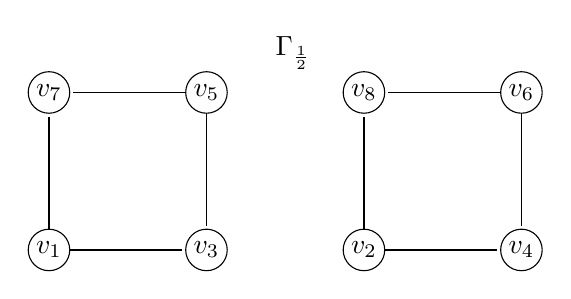
\begin{tikzpicture}[shorten >=1pt,auto,node distance=2cm,
thin,main node/.style = {circle,draw, inner sep = 0pt, minimum size = 15pt}]

\node[main node,fill=white] (1) {$v_1$};
\node[main node,fill=white] [right of = 1](2) {$v_3$};
\node[main node,fill=white] [above of = 1](3) {$v_7$};
\node[main node,fill=white] [above of =2](4) {$v_5$};
\node[main node,fill=white] [right of =2](5) {$v_2$};
\node[main node,fill=white] [right of = 5](6) {$v_4$};
\node[main node,fill=white] [above of = 5](7) {$v_8$};
\node[main node,fill=white] [above of =6](8) {$v_6$};
\node at (3.1,2.5) (9) {$\Gamma_{\frac{1}{2}}$};

\path[-]
(1) edge node {} (2)
edge node {} (3)
(4) edge node {} (3)
edge node {} (2)
(5) edge node {} (6)
edge node {} (7)
(8) edge node {} (7)
edge node {} (6);
\end{tikzpicture}\]
Similarly, if we instead consider $U_2$ as our projective design, $\Gamma_{\frac{\sqrt{2}}{2}}$ is given below.
\[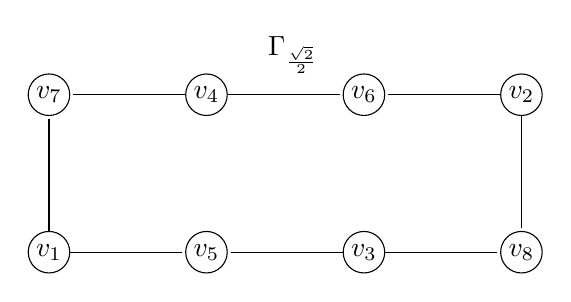
\begin{tikzpicture}[shorten >=1pt,auto,node distance=2cm,
	thin,main node/.style = {circle,draw, inner sep = 0pt, minimum size = 15pt}]
	
	\node[main node,fill=white] (1) {$v_1$};
	\node[main node,fill=white] [right of = 1](2) {$v_5$};
	\node[main node,fill=white] [above of = 1](3) {$v_7$};
	\node[main node,fill=white] [above of =2](4) {$v_4$};
	
	\node[main node,fill=white] [right of =2](5) {$v_3$};
	\node[main node,fill=white] [right of = 5](6) {$v_8$};
	\node[main node,fill=white] [above of = 5](7) {$v_6$};
	\node[main node,fill=white] [above of =6](8) {$v_2$};
	\node at (3.1,2.5) (9) {$\Gamma_{\frac{\sqrt{2}}{2}}$};
	
	\path[-]
	(1) edge node {} (2)
	edge node {} (3)
	(4) edge node {} (3)
	edge node {} (7)
	(5) edge node {} (6)
	edge node {} (2)
	(8) edge node {} (7)
	edge node {} (6);
\end{tikzpicture}\]
Thus $U_1$ and $U_2$ are non-isomorphic as their corresponding graphs are non-isomorphic double covers of $C_4$. Even further, define the five relations $R_0,\dots,R_4$ via the inner products $1$, $\alpha$, $0$, $-\alpha$, and $-1$ respectively so that, for instance, $(x,y)\in R_2$ if and only if the corresponding vectors are orthogonal. These four relations satisfy all the requirements of an association scheme except for possibly the existence of intersection numbers. In the case of the projective double $U_1$, we find that even though $(v_1,v_5)\in R_2$,
\[\left\vert\left\{v_x : (v_x,v_1),(v_5,v_x)\in R_{\alpha}\right\}\right\vert\neq\left\vert\left\{v_x : (v_x,v_1),(v_4,v_x)\in R_{\alpha}\right\}\right\vert.\]
However the projective double $U_2$ has well-defined intersection numbers and we find that the columns of $U_2$, along with the relations $R_0,\dots,R_4$, give the association scheme $C_8$.
\end{example}
As one might expect, there are many graphs for which we cannot find a projective double in the dimension given by the independence number. In other words, Proposition \ref{cocliquebnd} is often not tight. To see an example, consider the following proposition

\begin{prop}
	Let $\Gamma$ be a complete multipartite graph with $w$ parts of size $v$. Let $U$ be the matrix with columns corresponding to a projective double of $\Gamma$ where $\text{rank}\left(U\right) = \alpha\left(\Gamma\right) = v$. Then a subset of the columns of $U$ form a set of $w$ mutually unbiased bases in $\mathbb{R}^v$.\qed
\end{prop}
\begin{proof}
	Follow the same proof as in Proposition \ref{cocliquebnd}, however only consider one line from each antipodal pair. Noting that non orthogonal vectors must have inner product $\pm\alpha$, the result is immediate.
\end{proof}
\begin{cor}
	Let $\Gamma = K_{2\times t}$ for $t\neq 0\mod 4$. $\Gamma$ does not have a projective double in $\mathbb{R}^\alpha$ for $\alpha = \alpha\left(\Gamma\right)$.
\end{cor}
\begin{proof}
	If $K_{2\times t}$ had a bipartite double, then it would be a set of two mutually unbiased bases in $\mathbb{R}^t$. This is only possible when $t$ is a multiple of $4$.
\end{proof}

\section{Association schemes from projective doubles}
Example \ref{doublecoverc4} provides a projective double which naturally gives an association scheme on the vectors. In this section we consider which graphs may produce such an association scheme and some properties of the association scheme which arise. First, let $L$ be a projective double of some graph $\Gamma$ and let $G$ be the Gram matrix of $L$; that is the matrix whose entry in row $i$ and column $j$ is $\left<\ell_i,\ell_j\right>$. We denote by $\left<G\right>_\circ$ the vector space of matrices generated by $G$ using entrywise products. Note that the adjacency matrices of each graph $\Gamma_{\theta}$ for $\theta\in\left\{\pm 1,\pm \alpha,0\right\}$ are all contained in $\left<G\right>_{\circ}$. Thus $\left<G\right>_\circ$ is a Bose-Mesner algebra if and only if it is closed under standard matrix multiplication. If this occurs, we say $L$ induces the corresponding 4-class association scheme. Thus, from example \ref{doublecoverc4}, the association scheme $C_8$ is induced by the columns of $U_2$. We similarly define $\left<A\right>_*$ for any matrix $A$ and note that this algebra is closed under Schur products if and only if it is a Bose-Mesner algebra.

Now, a \emph{strongly regular graph} (see \cite{Brouwer1989}) with parameters $(v,k,\lambda,\mu)$ is a $k$-regular graph with $v$ points where every pair of adjacent vertices have exactly $\lambda$ neighbors in common while distinct non-adjacent vertices have $\mu$ neighbors in common. Using the terminology of association schemes, a strongly regular graph is a 2-class association scheme with parameters $k = p^0_{11}$, $\lambda = p^1_{11}$ and $\mu = p^2_{11}$.

\begin{prop}\label{projnec}
	A projective double of a simple graph $\Gamma$ induces an association scheme only if $\Gamma$ is strongly regular.
\end{prop}
\begin{proof}
	We will prove our result by showing that $\overline{\Gamma}$, the complement of $\Gamma$, is strongly regular. Let $v = \vert V\Gamma\vert$ and $L = \left\{\ell_1,\dots,\ell_{2v}\right\}$ with the projective mapping $\phi:L\rightarrow V\Gamma$. First let $R_0,\dots,R_4$ be the relations of the association scheme induced by $L$ where $R_2$ is given by orthogonality, $R_0$ is the identity relation, and the remaining relations are given by the inner products $\alpha,-\alpha,$ and $-1$ respectively. Next, $\phi(\ell)=\phi(\ell^\prime)$ if and only if $\ell=-\ell^\prime$. Thus for distinct vertices $u,w\in V\Gamma$, $u\not\sim w$ if and only if $\phi^{-1}(w)\subset \phi^{-1}(u)^\perp$. Then the number of vertices not adjacent to $u$ is half the number of vectors orthogonal to either vector in $\phi^{-1}(u)$; this value is $\frac{1}{2}p^0_{22}$. Similarly, assuming $u\not\sim w$, the number of vertices adjacent to neither $u$ nor $w$ must be half the number of vectors orthogonal to any pair of vectors, one from $\phi^{-1}(v)$ and the other from $\phi^{-1}(w)$; that is, $\frac{1}{2}p^2_{22}$. Similarly, assume $v\sim w$ and we find the number of vertices adjacent to neither $v$ nor $w$ must be $\frac{1}{2}p^1_{22} = \frac{1}{2}p^3_{22}$. Thus $\overline{\Gamma}$ is strongly regular with parameters $(\vert\Gamma\vert,\frac{1}{2}p^0_{22},\frac{1}{2}p^{2}_{22},\frac{1}{2}p^1_{22})$.
\end{proof}

This proposition tells us that we must only consider strongly regular graphs if we wish to find projective doubles which induce association schemes. Note that the converse of Proposition \ref{projnec} is certainly not true; the first projective double of Example \ref{doublecoverc4} does not result in an association scheme even though $C_4$ is strongly regular. Thus we will look for further necessary or sufficient conditions for a projective double to induce an association scheme. Before we continue, we review a few details of strongly regular graphs which will be useful for us.

Let $\Gamma$ be a strongly regular graph with parameters $(v,k,\lambda,\mu)$. Let $R_1$ be the relation given by adjacency in $\Gamma$ and define parameters $r,s,f,g$ so that the spectrum of $\Gamma$ is $k^1,r^f,s^g$. Using the first and second orthogonality relations (Lemma \ref{orthorels}) we find the first and second eigenmatrices of the association scheme are:
\begin{equation}\label{PQsrg}P = \left[\begin{array}{ccr}
1 & k & v-k-1\\
1 & r & -(r+1)\\
1 & s & -(s+1)
\end{array}\right],\qquad Q = \left[\begin{array}{ccc}
1 & f & g\\
1 & \frac{fr}{k} & \frac{gs}{k}\\
1 & \frac{f(1+r)}{k+1-v} & \frac{g(1+s)}{k+1-v}
\end{array}\right].\end{equation}
From \cite{Brouwer1989}, we find that the parameters $k,r,$ and $s$ are sufficient to define all other variables as long as $k+rs\neq 0$.
\begin{thm}\cite[Theorem.~1.3.1.(iii,vi)]{Brouwer1989} Whenever $k+rs>0$, the parameters of a strongly regular graph may be expressed in terms of $r$, $s$, and $k$ with $g = v-f-1$:
	\[\mu = k+rs, \qquad v = \frac{(k-r)(k-s)}{\mu},\qquad \lambda = \mu+r+s,\qquad f = \frac{(s+1)k(k-s)}{\mu(s+r)}.\]
\end{thm}
The association scheme structure allows us to improve on the naive upper bound given in Corollary \ref{regnaive} by using the techniques discussed in Section \ref{equilines}.
\begin{thm}
	Let $\Gamma$ be a strongly regular graph with spectrum $k^1,r^f,s^g$ $(r>s)$. There exists a projective double of $\Gamma$ in $\mathbb{R}^{f+1}$.
\end{thm}
\begin{proof}
	Let $A_0$, $A_1$, and $A_2$, be the adjacency matrices of the identity graph, $\Gamma$, and $\overline{\Gamma}$ respectively. From equation \eqref{PQsrg}, $E_1 = \frac{1}{v}\left(fA_0 + \frac{fr}{k}A_1 + \frac{f(1+r)}{k+1-v}A_2\right)$. Then 
	\[G = \frac{(1+r)}{v-k-1}E_0 + \frac{1}{f}E_1 = \left(\frac{v+r-k}{v(v-k-1)}\right)A_0 +\left(\frac{k+r(v-1)}{v(v-k-1)}\right)A_1\]
	is a $v\times v$ positive semi-definite matrix with rank $1+f$ with the innerproducts we seek. We may then find a matrix $U$ such that $\left(\frac{v(v-k-1)}{v+r-k}\right)G = U^TU$, that is, the columns of $U$ are unit vectors in $\mathbb{R}^{1+f}$ such that $u_i\perp u_j$ if and only if the corresponding points in $X$ are related by $R_2$. Then $L = \left\{\pm u_1,\dots,\pm u_v\right\}$ is a projective double of $\Gamma = \Gamma(X,R_1)$ where $u_i$ is the $i^\text{th}$ column of $U$.
\end{proof}
Note that this construction does not induce a 4-class association scheme. We see this by noting that all off diagonal entries in $G$ must be positive. Thus we may split our projective design into two sets $L^+$ and $L^-$ where $L^+$ contains all the columns of $U$ and $L^-$ contains their negatives. Then for vectors $u\perp v$, the number of vectors $w$ such that $\left<v,w\right> = \left<u,w\right>=\alpha$ could be either $0$ (if $v\in L^+$ and $u\in L^-$) or $\lambda$ (if $v,w\in L^+$). Thus this value is not solely dependent on the inner product $\left<u,v\right>$ and $p^2_{11}$ is not well defined. While this does not solve our question of which projective doubles induce association schemes, it does provide us with a better upper bound on the dimension needed for strongly regular graphs. For example, this gives a projective double of the Petersen graph in dimension $5$ while Corollary \ref{regnaive} produces one in dimension $9$. Now consider the following theorem of Delsarte.

\begin{thm}\cite{Delsarte1973} \label{delsarte}
	Let $\Gamma$ be a strongly regular graph with $v$ vertices, valency $k$, and smallest eigenvalue $s$. If $C$ is a coclique of $\Gamma$, then
	\[\vert C\vert\leq v\left(1-\frac{k}{s}\right)^{-1}, \]
	with equality if and only if every vertex $\gamma\notin C$ has the same number of neighbors (namely $-s$) in $C$.\qed
\end{thm}
We will refer to a \emph{Delsarte coclique} as a coclique for which this bound is tight. This theorem, along with Proposition \ref{cocliquebnd}, gives a lower bound on the dimension of any projective double in terms of the spectrum whenever $\Gamma$ contains a Delsarte coclique. Further, we may use the final line of Theorem \ref{delsarte} to learn more information about any projective double achieving this bound.
\begin{cor}\label{snegsquare}
	Let $\Gamma$ be a nonempty strongly regular graph with $v$ vertices, valency $k$ and smallest eigenvalue $s$ which contains a Delsarte coclique $C$. Then any projective double in $\mathbb{R}^{\vert C\vert}$ has inner product $\alpha=\sqrt{-s}$. Further, either $\Gamma$ is complete bipartite or $\alpha^{-1}\in \mathbb{Z}$.
\end{cor}
\begin{proof}
	Let $L$ be the projective double of $\Gamma$ in $\mathbb{R}^{\vert C\vert}$ with inner product $\alpha$. Further, let $\ell_1,\dots,\ell_{\vert C\vert}$ be vectors in $L$ such that the set $\left\{\phi(\ell_1),\dots,\phi(\ell_{\vert C\vert})\right\}$ is a Delsarte coclique. Then $\left\{\ell_1,\dots,\ell_t\right\}$ forms an orthonormal basis for $\mathbb{R}^{\vert C\vert} = \text{span}(L)$. Let $a\in L$ be given with $\phi(a)\notin C$. By Theorem \ref{delsarte}, $\phi(a)$ must be adjacent to exactly $-s$ points in $C$ and thus, reordering the vectors and replacing $\ell_i$ with $-\ell_i$ as needed, we may assume $\left<a,\ell_i\right> = \alpha$ for $1\leq i\leq -s$. Therefore $a = \sum_{i=1}^{-s} \alpha\ell_i$ implying that $-s\alpha^2 = 1$ and thus $s = -\alpha^{-2}$. Now, as long as $\Gamma$ is not complete bipartite, there must be another vector $b\in L$ for which $\phi(b)\notin C$ and $\phi(b) \sim\phi(a)$; assume $\left<b,a\right> = \alpha$ taking $-b$ if needed. We again find that $\phi(b)$ is adjacent to exactly $-s$ vertices in $C$; let $h$ be the number of vertices adjacent to both $a$ and $b$. Without loss of generality $b =  \sum_{i=1}^{h} \beta_i\ell_i + \sum_{i=-s+1}^{-2s-h}\alpha\ell_i$ where $\beta_i = \pm\alpha$. Thus $\left<a,b\right> = (p-q)\alpha^2$ where $p$ is the number of vectors in $\left\{\ell_1,\dots,\ell_h\right\}$ with $\left<b,\ell_i\right> = \left<a,\ell_i\right>$ and $q = h-p$. However, since $a$ and $b$ have inner product $\alpha$, this implies $\alpha^{-1} = p-q$.
\end{proof}
While this theorem does not provide information about projective doubles of strongly regular graphs without Delsarte cocliques, there are many common examples which contain these cocliques for which we may apply our theorem. For instance, consider the following result.
\begin{cor}
	There do not exist projective doubles for either the Petersen graph in $\mathbb{R}^4$ or the 9-Paley graph in $\mathbb{R}^3$. 
\end{cor}
\begin{proof}
	Recall that the Petersen graph has 10 vertices, valency 3, and smallest eigenvalue -2. Thus a Delsarte coclique has size $\nicefrac{10}{\left(1+\frac{3}{2}\right)} = 4$; we may verify quickly that such a coclique exists. Thus Corollary \ref{snegsquare} tells us a projective double of the Petersen graph in $\mathbb{R}^4$ would require that $\sqrt{-s}$ is an integer, which is of course false. Similarly the 9-Paley graph has 9 vertices, valency 4, and smallest eigenvalue -2. Using the same reasoning noting that here a Delsarte coclique has size 3, gives our result.
\end{proof}
It is worth pointing out that the points of the dodecahedron are often considered a projective double of the Peterson graph; contradicting the above result. In fact, the dodecahedron is a 4-distance antipodal set of size 20 with a mapping from these antipodal points to the vertices of the Petersen graph where the angle between two lines depends only on whether or not their images are adjacent. The problem with this construction is that orthogonal lines map to adjacent points in the Petersen graph, rather than non-adjacent points. Thus we consider the dodecahedron a projective double of the complement of the Petersen graph. This complement has valency 6 and smallest eigenvalue -2, requiring a Delsarte coclique to have size $2$. Thus Corollary \ref{snegsquare} requires nothing of a projective double in $\mathbb{R}^3$.

The following is a conjecture concerning necessary and sufficient conditions for $L$ to induce an association scheme.

\begin{conj}
	Let $\Gamma$ be a strongly regular graph with $v$ vertices, valency $k$, and smallest eigenvalue $s$. A projective double of $\Gamma$ in dimension $m<v$ induces an association scheme if and only if $m = v\left(1-\frac{k}{s}\right)^{-1}$.
\end{conj}
We prove a weaker version of one direction here.
\begin{thm}
	Let $\Gamma$ be a strongly regular graph with $v$ vertices, valency $k$, and smallest eigenvalue $s$. Let $L$ be a projective double of $\Gamma$ in dimension $m<v$ with inner product $\alpha$. $L$ induces an association scheme only if $m = v\left(1+k\alpha^2\right)^{-1}$. Further, either $\text{rank}\left(G\circ G\right)=v$ or the induced scheme is $Q$-bipartite and $s=-\alpha^{-2}$.
\end{thm}
\begin{proof}
	We prove this by building the $Q$ matrix of the resultant scheme. First let $\BMA = \left<G\right>_\circ$ and $\BMB = \left<A_\Gamma\right>_*$ where $A_\Gamma$ is the adjacency matrix of $\Gamma$. Since $G$ has five distinct values, $\BMA$ must be a 4-class association scheme with basis matrices $A_0,A_1,A_2,A_3,$ and $A_4$ corresponding to the values $1,\alpha,0,-\alpha,$ and $-1$. By definition of the projective double, we find that $R_0\cup R_4$ gives a system of imprimitivity where $\BMB$ is the quotient of $\BMA$. Since $\cI = \left\{0,4\right\}$, the matrix $A_0+A_4$ must be one basis matrix; the other two matrices are $A_1+A_3$ and $A_2$. Further there exist three basis idempotents of $\BMA$, call them $E_0$, $E_2$, and $E_4$, which span this same subalgebra. Since this subalgebra is closed under matrix multiplication, yet $A_1$ is not in this algebra, we must have $Q_{1j}=Q_{3j}$ for $j\in\left\{0,2,4\right\}$. Similarly $Q_{0j}=Q_{4j}$ for $j\in\left\{0,2,4\right\}$. Further, since our quotient map $\tilde{\psi}:\text{span}\left\{E_0,E_2,E_4\right\}\rightarrow \BMB$ preserves entrywise products, we must have
	\[\frac{Q_{12}}{\vert X\vert}\tilde{\psi}(A_1+A_2) =\tilde{\psi}(E_2\circ(A_1+A_2)) = \tilde{\psi}(E_2)\circ\tilde{\psi}(A_1+A_2)= \frac{\tilde{Q}_{12}}{\vert X\vert}\tilde{\psi}(A_1+A_2) \]
	and thus $\tilde{Q}_{12} = Q_{12} = Q_{32}$. We find similar expressions for all entries in columns $0$, $2$, and $4$ of $Q$. Equation \eqref{PQsrg} tells us that the second eigenmatrix of $\BMB$ is
	\[\tilde{Q} = \left[\begin{array}{ccc}
	1 & f & g\\
	1 & \frac{fr}{k} & \frac{gs}{k}\\
	1 & \frac{f(1+r)}{k+1-v} & \frac{g(1+s)}{k+1-v}
	\end{array}\right]\]
	and thus the second eigenmatrix of $\BMA$ must have the form
	\[Q = \left[\begin{array}{crcrc}
	1 & * & f & * & g\\
	1 & * & \frac{fr}{k}  & * & \frac{gs}{k}\\
	1 & * & \frac{f(r+1)}{k+1-v}  & *& \frac{g(1+s)}{k+1-v}\\
	1 & * & \frac{fr}{k} & * & \frac{gs}{k}\\
	1 & * & f & * & g\\
	\end{array}\right]\]
	Let $n_1$ and $n_3$ be the remaining two multiplicities corresponding to $E_1$ and $E_3$ respectively. Since $1+f+g=v$ and $\vert X\vert = 2v$, we must have $n_1+n_3 = v$. Now, by construction, $G = A_0 + \alpha A_1 -\alpha A_3 -A_4$ and therefore the top left entry of $GE_2$ is given by
	\[\left[GE_2\right]_{11} = \frac{1}{\vert X\vert}\left(f+k\left(\frac{fr}{k}\right)\alpha - k\left(\frac{fr}{k}\right)\alpha -f\right) = 0.\]
	Similarly, the top left entries of both $GE_4$ and $GE_0$ are also $0$. This can only happen if $GE_i = 0$ for $i\in\left\{0,2,4\right\}$. Thus there exists constants $c_1$, and $c_3$ such that $G = c_1E_1+c_3E_3$. Since $m<v$, we must have either $c_1$ or $c_3$ to be 0; without loss of generality assume $c_3 =0$. This gives us that $n_1 = m$ and $G = \frac{\vert X\vert}{m}E_1$. Therefore $G^2 = \frac{\vert X\vert^2}{m^2}E_1$ and we find
	\[\left[G^2\right]_{11} = 2\left(1+k\alpha^2\right) = \frac{\vert X\vert}{m}\]
	implying $m = v\left(1+k\alpha^2\right)^{-1}$.
	
	Now, we may return to our $Q$ matrix and fill in the entries of the first column. Further, the orthogonality relations (Lemma \ref{orthorels}) tell us that $\sum_{j}Q_{ij} = \delta_{0j}\vert X\vert$. Using the same fact for $\tilde{Q}$, we may find the final column as well. 
	\[Q = \left[\begin{array}{crccc}
	1 & m & f & v-m & g\\
	1 & m\alpha & \frac{fr}{k}  & -m\alpha & \frac{gs}{k}\\
	1 & 0 & \frac{f(r+1)}{k+1-v}  & 0& \frac{g(1+s)}{k+1-v}\\
	1 & -m\alpha & \frac{fr}{k} & m\alpha & \frac{gs}{k}\\
	1 & -m & f & m-v & g\\
	\end{array}\right]\]
	Since we now have the entire $Q$ matrix, we may use Lemma $\ref{kitchensink}$ $(xiii^\prime)$ to find the Krein parameters of our scheme. In particular we find that $q^3_{11} = q^4_{12} = 0$ as well as
	\[\begin{aligned}q^2_{11} &= \frac{1}{2v f}\sum_{h=0}^d\left(k_hQ_{h1}Q_{h1}Q_{h2}\right) = \frac{m^2\left(1+\alpha^2r\right)}{v},\\
	q^3_{12} &= \frac{1}{2v (v-m)}\sum_{h=0}^d\left(k_hQ_{h1}Q_{h2}Q_{h3}\right) = \frac{mf\left(v-m(1+\alpha^2r)\right)}{v(v-m)},\\
	q^4_{13} &= \frac{1}{2v g}\sum_{h=0}^d\left(k_hQ_{h1}Q_{h3}Q_{h4}\right) = \frac{m\left(v-m(1+\alpha^2s)\right)}{v}.\\	
	\end{aligned}\]
	Noting that $v- m(1+\alpha^2r)>v-m(1+\alpha^2k) = 0$ as long as $r\neq k$ ($\Gamma$ is not complete) we have all three Krein parameters nonzero. Thus $\BMA$ is $Q$-polynomial if and only if $q^{4}_{11}=0$. Calculating this similarly, we find
	\[q^4_{11} = \frac{1}{2v g}\sum_{h=0}^d\left(k_hQ_{h1}Q_{h1}Q_{h4}\right) = \frac{m^2g\left(1+\alpha^2s\right)}{v}.\]
	Thus $q^4_{11}=0$ if and only if $s = -\alpha^{-2}$. Finally since $q^0_{11},q^2_{11}>0$, we find that $\text{rank}(G\circ G) = 1+f+g=v$ if $q^4_{11}>0$ and $\text{rank}(G\circ G) = 1+f<v$ otherwise.
\end{proof}
\begin{cor}
	Let $\Gamma$ be a strongly regular graph with $v$ vertices, valency $k$, and smallest eigenvalue $s$ which contains a Delsarte coclique. Then the association scheme induced by any projective double of $\Gamma$ in dimension $m<v$ is $Q$-bipartite.
\end{cor}
\begin{proof}
	Repeat the previous proof noting that either $q^4_{11}=0$ or $-s\alpha^{2}>1$. The latter implies $(1+k\alpha^{-2})^{-1}<(1-ks)^{-1}$ forcing $m <v(1-ks)^{-1}$, violating Lemma \ref{cocliquebnd}.
\end{proof}
\section{4-class $Q$-bipartite association schemes}



\begin{restatable*}{thm}{fourclasssixzero}\label{thm60}
	Suppose we have a feasible parameter set for a $4$-class association scheme which is $Q$-bipartite but not $Q$-antipodal. Let $k=P_{01}$, $r=P_{21}$, and $s=P_{41}$ where $P$ is the first eigenmatrix using the natural ordering. Then the scheme is realizable only if $s=-n^2$ for some integer $n>1$ and
	\[15n^4(2n^2-3)r^2 + (n^6-45kn^2+76k)n^2r+k(16k+n^6)(n^2-2)\geq 0.\]
\end{restatable*}

In this chapter we investigate the specific case of $4$-class $Q$-bipartite schemes. LeCompte et al.\ \cite{LeCompte2010} proved that real mutually unbiased bases are equivalent to 4-class $Q$-bipartite schemes which are also $Q$-antipodal. This extra system of imprimitivity arises as one of the quotient graphs is a union of cliques, the other being complete multipartite. Here, we will instead restrict ourselves to the case where our association schemes are not $Q$-antipodal thus assuming that both quotient graphs are connected. We will begin by showing that the parameters of any such scheme are determined completely by three integral parameters and then recast Theorem \ref{cometricbnds} in terms of these three parameters. Let $(X,\mathcal{R})$ be a 4-class $Q$-bipartite association scheme with $Q$-polynomial ordering $E_0,E_1,\dots,E_4$ and natural ordering $A_0,A_1,\dots A_4$. We know from Theorem \ref{suzuki} that the quotient of $(X,\mathcal{R})$ has exactly two non-trivial relations and thus must be strongly regular. Let $(v,k,\lambda,\mu)$ be the parameters of the quotient strongly regular graph which contains $R_1$ as a subgraph. Let $k>r>s$ be the eigenvalues of this SRG with corresponding multiplicities $1$, $f$, and $g$. Since $(X,\mathcal{R})$ is not $Q$-antipodal, we must have $k>r$ and $s>-k$. The $Q$ matrix of this SRG will be
\[\tilde{Q} = \left[\begin{array}{ccc}
1 & f & g\\
1 & \frac{fr}{k} & \frac{gs}{k}\\
1 & \frac{f(1+r)}{k+1-v} & \frac{g(1+s)}{k+1-v}
\end{array}\right].\]
We may use this information to build the first and second eigenmatrices of our $4$-class $Q$-bipartite scheme as follows.
\begin{thm}
	\label{Pmat}
	Let $(X,\mathcal{R})$ be a 4-class $Q$-bipartite association scheme with relations ordered naturally. Let the quotient SRG have $v$ vertices and spectrum $k^1,r^f,s^g$ with $k>r>s$. Then the first and second eigenmatrices are as follows:
	\[P = \left[\begin{array}{crcrr}
	1 & k & 2(v-1-k) & k & 1\\
	1 & \frac{k}{n} & 0 & -\frac{k}{n} & -1\\
	1 & r& -2(1+r) & r & 1\\
	1 & -n & 0 & n & -1\\
	1 & s & -2(s+1) & s & 1\\
	\end{array}\right]\qquad Q = \left[\begin{array}{crcrc}
	1 & m & f & \frac{mk}{n^2} & g\\
	1 & \frac{m}{n} & \frac{fr}{k}  & -\frac{m}{n} & \frac{gs}{k}\\
	1 & 0 & \frac{f(r+1)}{k+1-v}  & 0& \frac{g(1+s)}{k+1-v}\\
	1 & -\frac{m}{n} & \frac{fr}{k} & \frac{m}{n} & \frac{gs}{k}\\
	1 & -m & f & \frac{mk}{n^2} & g\\
	\end{array}\right]\]
	where $s = -n^2$.
\end{thm}
\begin{proof}
	We begin by building all of $Q$ and then employ the use of our orthogonality properties. Note that column 0 of $Q$ comes by definition. From Theorem [\cite{Brouwer2003},\cite{Martin2007}], $Q_{1,1} = -Q_{3,1}\neq 0 = Q_{2,1}$, so we define $n = \frac{m}{Q_{1,1}} = -\frac{m}{Q_{3,1}}$ and column 1 is given. The first three entries of columns $2$ and $4$ follow from the parameters of our quotient scheme while the remaining two entries of each columns follow from Corollary \ref{evenpoly}. Finally column 3 may be found using the first orthogonality condition (specifically that $\displaystyle{\sum_j Q_{ij} = \vert X\vert\delta_{i0}}$). From here we have that 
	\[Q = \left[\begin{array}{crccc}
	1 & m & f & v-m & g\\
	1 & \frac{m}{n} & \frac{fr}{k}  & -\frac{m}{n} & \frac{gs}{k}\\
	1 & 0 & \frac{f(r+1)}{k+1-v}  & 0& \frac{g(1+s)}{k+1-v}\\
	1 & -\frac{m}{n} & \frac{fr}{k} & \frac{m}{n} & \frac{gs}{k}\\
	1 & -m & f & m-v & g\\
	\end{array}\right],\]
	matching our theorem in all but two places.	Since we have ordered the relations using the natural ordering, the valencies of our relations are given by $[1,k,2(v-1-k),k,1]$. This allows us to derive an expression for $q_{01}^1$ using \cite[Theorem.~2.3.2.]{Brouwer1989} which gives
	\[q_{ij}^k = \frac{1}{\vert X\vert m_k}\sum_{l=0}^d\left(v_lQ_{li}Q_{lj}Q_{lk}\right)\]
	where $m_k$ and $v_l$ are the multiplicities and valencies of the $k^\text{th}$ and $l^\text{th}$ relations respectively. We find that $q_{01}^1 = \frac{1}{2vm}\left(2m^2+\frac{2km^2}{n^2}\right)$, however we know from Theorem \ref{kreinidentities} that $q_{01}^1=1$, resulting in $\frac{km}{n^2} = v-m$. This completes our proof for the second eigenmatrix and we may use the second orthogonality condition to find $P$ noting that the first row of $P$ is the valencies of our relations. Thus
	\[P = \left[\begin{array}{crcrr}
	1 & k & 2(v-1-k) & k & 1\\
	1 & \frac{k}{n} & 0 & -\frac{k}{n} & -1\\
	1 & r& -2(1+r) & r & 1\\
	1 & -n & 0 & n & -1\\
	1 & s & -2(s+1) & s & 1\\
	\end{array}\right].\]
	We again use our equation for Krein parameters one more time to find $q_{11}^4 = \frac{mg(n^2+s)}{n^2v}$. Since $q_{11}^4=0$ due to our cometric property, we have that $s = -n^2$.
\end{proof}
\begin{cor}
	The parameters of a 4-class $Q$-bipartite scheme are uniquely determined by the eigenvalues of the quotient SRG.
\end{cor}
\begin{proof}
	Our first eigenmatrix only requires $v,k,r,s,$ and $n$. However since $n>0$ (from the natural ordering of relations), $n = \sqrt{-s}$. Further \cite{Brouwer1989} states that  $v = \frac{(k-r)(k-s)}{k+rs}$. 
\end{proof}
Before moving to examine the effect of Sch\"{o}nberg's theorem on 4-class $Q$-bipartite schemes, we mention a few parameter bounds arising from the feasibility conditions FC1-FC3 and show how they restrict the space of feasible parameters.
\begin{thm}
	\label{bounds}
	Suppose we have a feasible parameter set for a $4$-class association scheme which is $Q$-bipartite but not $Q$-antipodal. Let $k=P_{01}$, $r=P_{21}$, and $s=P_{41}$ where $P$ is the first eigenmatrix using the natural ordering. The following must hold with $n:=\sqrt{-s}$ and $\mu=k+rs$:
	\begin{enumerate}[label=(\roman*)]
		\item $\mu\geq n(r+n)$,
		\item $n\vert \mu$ and $n\vert k$,
		%\item $r\leq \frac{k-n^2}{n(n+1)}$,
		\item $r\geq \frac{2k}{3n^2}-\frac{n^2}{3}$,
		\item $kn^2(n^2-1)\geq \mu(n^2+r)$
	\end{enumerate}
	Further, $n$ is an integer greater than 1.
\end{thm}
\begin{proof}
	First note that $k$, $r$, and $s$ are the eigenvalues of a strongly regular graph and thus integral (we assume here that the SRG is not a conference graph). For $(i)$ and $(ii)$, note that	$p_{13}^1 = \frac{(n-1)(\mu-n(r+n))}{2n}$. FC2 tells us that this must be a non-negative integer, and therefore we must either have $-s = n = 1$ or $\mu-n(r+n)\geq0$. As $s=-1$ implies our SRG is a union of cliques (and thus $(X,\mathcal{R})$ is $Q$-antipodal), we may ignore this case and $(i)$ follows. Since $\gcd(n,n-1)=1$, we have that $n\vert (\mu-n(r+n))$ forcing $n\vert \mu$ and since $k=\mu+rn^2$, $(ii)$ follows. Next, $(iii)$ follows from the absolute bound $1+f \leq \frac{m(m+1)}{2}$ giving us $n^4+3n^2r-2k\geq 0$. Using another absolute bound, $(iv)$ follows from $\frac{v}{m}\leq f$. Finally, since $n = \sqrt{-s}$, if $n$ is not an integer, then columns one and three of $Q$ must be irrational. However Galois conjugation is an automorphism of our Bose-Mesner algebra and thus $E_0$, $E_3$, $E_2$, $E_1$, $E_4$ must be a second $Q$ polynomial ordering in this case, implying $q_{3,3}^4=0$. Using our $P$ and $Q$ matrices, we find that $q_{3,3}^4 = \frac{(k-r)(k+s)}{\mu}$. This means that whenever $n$ is irrational, either $r=k$ or $s = -k$, both of which imply $(X,\mathcal{R})$ is $Q$-antipodal.
\end{proof}

\begin{cor}
	\label{kbnds}
	Suppose we have a feasible parameter set for a $4$-class association scheme which is $Q$-bipartite but not $Q$-antipodal. Let $k=P_{01}$, $r=P_{21}$, and $s=P_{41}$ where $P$ is the first eigenmatrix using the natural ordering. Then
	\[\frac{k}{n^2}-1\leq \frac{(n+1)}{2}\left((n+1)(n^3-n-1)+\sqrt{(n-1)(n^7+3n^6+2n^5-4n^4-9n^3-3n^2+3n-1)}\right).\]
\end{cor}
\begin{proof}
	Using Theorem \ref{bounds}$(i)$ and $(iv)$, we have that $n(r+n)\leq \mu\leq \frac{kn^2(n^2-1)}{n^2+r}$. Using $\mu = k-rn^2$, these two inequalities give us
	\[\frac{k-n^4+\sqrt{n^8-2n^4k(2n^2+3)+k^2}}{2n^2}\leq r\leq \frac{k-n^2}{n(n+1)}.\]
	This implies that 
	\[k^2-n^2(n^5+2n^4-3n^2-3n+1)k+n^5(n^2+n-1)\leq0.\]
	When $k=1$ and $n>1$, the left hand side will be negative. Therefore this requires that $k$ is less than the positive root of this quadratic, giving us our bound.
\end{proof}
We now examine the bounds arising from Corollary \ref{Qbipbnds} as applied to our 4-class $Q$-bipartite association scheme. We begin by noting that $\theta_{31}\geq 0$ becomes Theorem \ref{bounds} $(i)$ when we use the parameters $k$, $r$, and $n$, thus making it equivalent to an absolute bound in this context. Next, we find that plugging in our parameters gives $\theta_{42}\geq 0$ and $\theta_{53}\geq 0$ if and only if $k\geq \frac{-rn^2}{n^2-2}$ and $k\geq -\frac{(3n^2-7)rn^2}{n^4-3n^2+6}$ respectively. Both of these bounds are vacuous since the right hand side will be negative for any choice of $n>1$. Finally one may show that $\theta_{31}\geq 0$ and $\theta_{60}\geq 0$ together imply $\theta_{51}\geq 0$ in the specific case of a 4-class $Q$-bipartite scheme. Therefore the only new restriction, not implied by FC1-FC3 is $\theta_{60}\geq 0$, resulting in the following theorem.
\fourclasssixzero
\begin{comment}\begin{thm}\label{thm60}
Suppose we have a feasible parameter set for a $4$-class association scheme which is $Q$-bipartite but not $Q$-antipodal. Let $k=P_{01}$, $r=P_{21}$, and $s=P_{41}$ where $P$ is the first eigenmatrix using the natural ordering. Then the scheme is realizable only if
\[15n^4(2n^2-3)r^2 + (n^6-45kn^2+76k)n^2r+k(16k+n^6)(n^2-2)\geq 0.\]
\end{thm}
\end{comment}
\begin{proof}
	Apply the parameters $k,r,$ and $s$ to Theorem \ref{Qbipbnds} $(v)$.
\end{proof}
We may pair this Theorem with Theorem \ref{bounds} to get the following corollary.
\begin{cor}\label{newkbnds}
	Suppose we have a feasible parameter set for a $4$-class association scheme which is $Q$-bipartite but not $Q$-antipodal. Let $k=P_{01}$, $r=P_{21}$, and $s=P_{41}$ where $P$ is the first eigenmatrix using the natural ordering. The following table gives an upper bound on the largest eigenvalue $k$ based on the smallest $s$ for $-4\leq s\leq 121$:
	\[\begin{tabular}{c|c|c|c|c|c|c|c|c|c|c}
	$n$ & 2 & 3 & 4 & 5 & 6 & 7 & 8 & 9 & 10 & 11\\\hline
	$k\leq$  & 56 & 891 & 5504 & 22297 & 85128 & 282828 & 867787 & 2609805 & 8468529 & 40926495\\
	\end{tabular}\]
\end{cor}
\begin{proof}
	Let $r_1\geq r_2$ be the two roots of $15n^4(2n^2-3)r^2 + (n^6-45kn^2+76k)n^2r+k(16k+n^6)(n^2-2)$. Then Theorem \ref{thm60} tells us that either $r\geq r_1$ or $r\leq r_2$. Pairing this with Theorem $\ref{bounds}$ we find that $r\geq r_1$ and $\mu\geq n(r+n)$ together restrict $k$ via
	\[\begin{aligned}	\frac{k}{n^3(n^2-1)}&\leq \frac{n^7+2n^6-3n^4-17n^3+45n^2+14n-76}{-2(n^4-13n^3+15n^2+12n-32)(n^2-1)}\\
	&\qquad+\frac{\sqrt{n^{10}+4n^9+6n^8+2n^7-35n^6+22n^5+145n^4-72n^2+32n+16}}{-2(n^4-13n^3+15n^2+12n-32)}.\end{aligned}\]
	Secondly, $r\leq r_2$ with $r\geq\frac{2k}{3n^2}-\frac{n^2}{3}$ implies that $k\leq \frac{3n^6-5n^4}{2}$. Taking the maximum of these two bounds for each $2\leq n\leq 11$ results in the values given in the table. In each case apart from $n=11$, this is a reduction from the bound given in Theorem \ref{kbnds}
\end{proof}
We conclude this chapter by noting the impact of Theorem \ref{thm60} on the feasible parameter space of 4-class $Q$-bipartite association schemes. In the table below we list the number of feasible schemes for a given $n>0$ when only considering conditions FC1, FC2, and FC3. We also list the number of feasible schemes when we include Theorem \ref{thm60} as a feasibility condition.
\[\begin{tabular}{c|c|c}\label{feasible4class}
$n$ & \# of feasible parameter sets & \# of feasible parameter sets satisfying Theorem \ref{thm60}\\\hline
2 & 6 & 5\\
3 & 60 & 44\\
4 & 223 & 140\\
5 & 473 & 334\\
6 & 1015& 701\\
7 & 1256& 952\\
8 & 2256& 1659\\
\end{tabular}\]
The following figures display the original feasibility conditions and the new bound due to $\theta_{60}\geq 0$. We display the graphs for $n=7$, noting that similar graphs may be generated for any $n>1$.
\begin{figure}[h]
	\begin{subfigure}[h]{0.5\textwidth}
		\includegraphics[scale=.5]{bounds7py.png}
	\end{subfigure}
	\begin{subfigure}[h]{0.5\textwidth}
		\includegraphics[scale=.5]{geg7.png}
	\end{subfigure}
	\caption[4-class $Q$-bipartite bounds]{These figures pertain to the case $n = 7$. On the left we have two absolute bounds and a bound due to the non-negativity of an intersection number. In green, we have plotted every parameter set which is feasible under FC1-FC3. On the right, we have replaced the bounds with the bound $\theta_{60}\geq 0$. Any parameter set contained within the parabola is not realizable.}
\end{figure}
\section{Connectivity of basis relations}
\chapter{Connectivity of basis relations}\label{connectivity}
\end{document}
